\documentclass[pdflatex,sn-mathphys-num]{sn-jnl}% Math and Physical Sciences Numbered Reference Style
%%\documentclass[pdflatex,sn-mathphys-ay]{sn-jnl}% Math and Physical Sciences Author Year Reference Style
%%\documentclass[pdflatex,sn-aps]{sn-jnl}% American Physical Society (APS) Reference Style
%%\documentclass[pdflatex,sn-vancouver-num]{sn-jnl}% Vancouver Numbered ReferFence Style
%%\documentclass[pdflatex,sn-vancouver-ay]{sn-jnl}% Vancouver Author Year Reference Style
%%\documentclass[pdflatex,sn-apa]{sn-jnl}% APA Reference Style
%%\documentclass[pdflatex,sn-chicago]{sn-jnl}% Chicago-based Humanities Reference Style

%%%% Standard Packages
%%<additional latex packages if required can be included here>

\usepackage{graphicx}%
\usepackage{multirow}%
\usepackage{amsmath,amssymb,amsfonts}%
\usepackage{amsthm}%
\usepackage{mathrsfs}%
\usepackage[title]{appendix}%
\usepackage{xcolor}%
\usepackage{textcomp}%
\usepackage{manyfoot}%
\usepackage{booktabs}%
\usepackage{algorithm}%
\usepackage{algorithmicx}%
\usepackage{algpseudocode}%
\usepackage{listings}%
%%%%

%% Revision marking: all modified/added text is shown in red.
%% For the final submission, replace the definition by \newcommand{\rev}[1]{#1}
\newcommand{\rev}[1]{\textcolor{red}{#1}}

%%%%%=============================================================================%%%%
%%%%  Remarks: This template is provided to aid authors with the preparation
%%%%  of original research articles intended for submission to journals published 
%%%%  by Springer Nature. The guidance has been prepared in partnership with 
%%%%  production teams to conform to Springer Nature technical requirements. 
%%%%  Editorial and presentation requirements differ among journal portfolios and 
%%%%  research disciplines. You may find sections in this template are irrelevant 
%%%%  to your work and are empowered to omit any such section if allowed by the 
%%%%  journal you intend to submit to. The submission guidelines and policies 
%%%%  of the journal take precedence. A detailed User Manual is available in the 
%%%%  template package for technical guidance.
%%%%%=============================================================================%%%%

%% as per the requirement new theorem styles can be included as shown below
\theoremstyle{thmstyleone}%
\newtheorem{theorem}{Theorem}%  meant for continuous numbers
%%\newtheorem{theorem}{Theorem}[section]% meant for sectionwise numbers
%% optional argument [theorem] produces theorem numbering sequence instead of independent numbers for Proposition
\newtheorem{proposition}[theorem]{Proposition}% 
%%\newtheorem{proposition}{Proposition}% to get separate numbers for theorem and proposition etc.

\theoremstyle{thmstyletwo}%
\newtheorem{example}{Example}%
\newtheorem{remark}{Remark}%

\theoremstyle{thmstylethree}%
\newtheorem{definition}{Definition}%

\raggedbottom
%%\unnumbered% uncomment this for unnumbered level heads

\begin{document}

\title[2‑D and 3‑D Neural Networks]{Patch‑Based Neural Networks for Learning Derivatives and Solving PDEs in 2‑D and 3‑D}

\author[1]{\fnm{Babak} \sur{Shiri}}\email{shiri@njtc.edu.cn}



\author*[2]{\fnm{Zahra} \sur{Alijani}}\email{Zahra.Alijani@osu.cz}
\author[3,4]{\fnm{Dumitru} \sur{Baleanu}}\email{dumitru.baleanu@lau.edu.lb}

\author[5]{\fnm{Juan} \sur{J.~Nieto}}\email{juanjose.nieto.roig@usc.es}
%juanjose.nieto.roig@usc.es


\affil[1]{Key Laboratory of Numerical Simulation of Sichuan Provincial Universities, School of Mathematics and Big Data, Neijiang Normal University, Neijiang, 641100, China}
\affil[2]{Institute for Research and Applications of Fuzzy Modeling, University of Ostrava, 30. dubna 22, Ostrava, 701 03, Czech Republic}
\affil[3]{Department of Computer Science and Mathematics, Lebanese American University, Beirut, 1102 2801, Lebanon}

\affil[4]{Institute of Space Sciences, Magurele-Bucharest, R 76900, Romania}



\affil[5]{CITMAga (Galician Centre for Mathematical Research and Technology)
Department of Statistics, Mathematical Analysis and Optimization
University of Santiago de Compostela
Santiago de Compostela, 15782 Spain}


\abstract{
Discrete derivative stencils are traditionally derived by hand from mathematical relations. In this work, patch‑based neural networks are presented to learn spatial derivative operators directly from training data, without manually constructing finite‑difference stencils. The proposed framework is formulated for two‑dimensional matrix fields and generalized to three‑dimensional tensor data. Network weights are obtained by solving linear systems, instead of relying on iterative gradient‑descent optimization. Backward local patches with constant replication padding are used to handle domain boundaries. The learned derivative operators are embedded within a marching scheme for solving first‑order partial differential equations. Consistency and convergence properties are investigated through numerical benchmarks. Results show that the learned operators achieve first‑order convergence on test functions. Stable numerical PDE solutions are obtained for example problems in both two and three spatial dimensions. A two‑layer corrector network is also tested to reduce approximation error, and structural constraints are introduced to stabilize three‑dimensional learned stencils.}


\keywords{Patch‑based neural networks, data‑informed derivative approximation, partial differential equations, multi‑dimensional tensor fields}

%%\pacs[JEL Classification]{D8, H51}

%%\pacs[MSC Classification]{35A01, 65L10, 65L12, 65L20, 65L70}

\maketitle

\section{Introduction}
Can we recover a discrete numerical operator directly from the known action of the operator on a set of basis functions, such as polynomials? This avoids manual derivation of stencil formulas.

Traditional numerical differentiation methods are knowledge-driven. They use fixed finite difference stencils or pre-defined governing equations. For a bivariate field $F_{ij}=F(X_i,Y_j)$ stored as a matrix, standard partial derivatives are computed as weighted sums along one axis only:
\begin{align}
\frac{\partial F_{ij}}{\partial X} &= \sum_{k} W_{ik} F_{kj}, \\
\frac{\partial F_{ij}}{\partial Y} &= \sum_{k} W_{kj} F_{ik},
\end{align}
where $W_{ik}$ and $W_{kj}$ are fixed weights derived by hand. These single-sum formulas only collect information along one axis. They cannot compute general directional derivatives that require coupled information from both spatial dimensions. To capture cross-axis spatial dependence, we use a bilinear double-sum form for the derivative at grid point $(n,m)$:
\begin{equation}
\frac{\partial F_{nm}}{\partial \boldsymbol{\xi}} = \sum_{k=1}^n\sum_{k'=1}^m W_{{n}k}^{L} F_{kk'} W_{k'{m}}^{R}.
\end{equation}
This is a backward scheme: the derivative at $(n,m)$ uses only data from grid points before $(n,m)$. A forward scheme can be built similarly using later grid entries. Instead of manually fixing weights, this motivates our data-driven two-dimensional neural network, which learns optimal $\boldsymbol{W}^{L}$ and $\boldsymbol{W}^{R}$ from paired input fields and their target derivative values.

Lightweight neural networks for visual tasks have seen extensive development. Core initialization and optimization techniques are well established \cite{xavier_glorot, heavy_init, kingma2014adam}. Foundational models including support vector machines \cite{Cortes1995}, multilayer perceptrons \cite{Rumelhart1986}, and convolutional networks \cite{Lecun1998, Krizhevsky2012} enable high-accuracy image classification. Recent neuromorphic and optoelectronic network designs target low-power edge computing hardware \cite{Li2023, Beyeler2013, Song2024}. Even so, lightweight architectures that fully preserve the native two-dimensional spatial structure of grid data remain open to improvement.

The standard matrix multiplication used in basic neural networks carries structural limitations relevant to our derivative approximation goal. Given input matrix $\boldsymbol{X}$ and learnable weight matrix $\boldsymbol{W}$, the output feature matrix is defined by
\[
\boldsymbol{Y} = \boldsymbol{W}\boldsymbol{X},
\]
with individual entries
\[
Y_{ij} = \sum_{p} W_{ip} X_{pj}.
\]
Each output entry $Y_{ij}$ depends only on the $j$-th column of $\boldsymbol{X}$. It ignores spatial information carried by other columns. This restricted information flow limits the model’s capacity to capture full two-dimensional spatial context.

To overcome this restriction, we construct network layers that apply separate linear transforms on the left and right sides of the input matrix. Consider an input matrix $\boldsymbol{X} \in \mathbb{R}^{\mu_1 \times \nu_1}$. Each layer maps this matrix to a new feature matrix $\boldsymbol{Z}^{[1]}$ of target dimension $\mu_2 \times \nu_2$. First, a left linear transform with learnable $\boldsymbol{W}^{[L1]} \in \mathbb{R}^{\mu_2 \times \mu_1}$ produces an intermediate matrix of size $\mu_2 \times \nu_1$. A complementary right multiplication with $\boldsymbol{W}^{[R1]} \in \mathbb{R}^{\nu_1 \times \nu_2}$ then adjusts the second spatial dimension. The layer is defined as
\begin{align}
\boldsymbol{Z}^{[L1]}_{\mu_2 \times \nu_1} &= \boldsymbol{W}^{[L1]}_{\mu_2 \times \mu_1} \boldsymbol{X}_{\mu_1 \times \nu_1} + \boldsymbol{B}^{[L1]}_{\mu_2 \times \nu_1}, \\
\boldsymbol{Z}^{[1]}_{\mu_2 \times \nu_2}  &= \boldsymbol{Z}^{[L1]}_{\mu_2 \times \nu_1} \boldsymbol{W}^{[R1]}_{\nu_1 \times \nu_2} + \boldsymbol{B}^{[R1]}_{\mu_2 \times \nu_2},
\end{align}
where $\boldsymbol{B}^{[L1]}$ and $\boldsymbol{B}^{[R1]}$ are learnable bias matrices. Substituting the first equation into the second gives the combined expression:
\[
\boldsymbol{Z}^{[1]}
=
\boldsymbol{W}^{[L1]} \boldsymbol{X} \boldsymbol{W}^{[R1]}
+ \boldsymbol{B}^{[L1]} \boldsymbol{W}^{[R1]}
+ \boldsymbol{B}^{[R1]}.
\]
The term $\boldsymbol{B}^{[L1]} \boldsymbol{W}^{[R1]}$ is independent of the input and can be merged into a single unified bias $\boldsymbol{B}^{[1]}$. The simplified pre-activation output becomes
\begin{equation}\label{6E}
\boldsymbol{Z}^{[1]}_{\mu_2 \times \nu_2}
=
\boldsymbol{W}^{[L1]}_{\mu_2 \times \mu_1}
\boldsymbol{X}_{\mu_1 \times \nu_1}
\boldsymbol{W}^{[R1]}_{\nu_1 \times \nu_2}
+ \boldsymbol{B}^{[1]}_{\mu_2 \times \nu_2}.
\end{equation}
An element-wise nonlinear activation function
\[
F^{[1]}: \mathbb{R}^{\mu_2 \times \nu_2} \to \mathbb{R}^{\mu_2 \times \nu_2}
\]
introduces nonlinearity, yielding the final layer output
\begin{equation}
\boldsymbol{Y}^{[1]}_{\mu_2 \times \nu_2}
=
F^{[1]}\bigl(\boldsymbol{Z}^{[1]}_{\mu_2 \times \nu_2}\bigr).
\end{equation}

For our derivative approximation task, the input $\boldsymbol{X}$ corresponds to a two-dimensional patch, and the target output reduces to a single scalar value. We therefore set $\mu_2=\nu_2=1$, which corresponds to estimating a derivative at a grid corner using information from the surrounding patch. The network simplifies to
\begin{equation}\label{8E}
\begin{split}
z^{[1]}
=&
\boldsymbol{W}^{[L1]}_{1 \times \mu_1}
\boldsymbol{X}_{\mu_1 \times \nu_1}
\boldsymbol{W}^{[R1]}_{\nu_1 \times 1}
+ b^{[1]}\\
=&\sum_{k=1}^{\nu_1}\sum_{p=1}^{\mu_1} W^{[L1]}_{1p}X_{pk}W^{[R1]}_{k1}+ b^{[1]}.
\end{split}
\end{equation}
Define a unified weight matrix $\boldsymbol{W}^{[u]}=(W^{[u]}_{ij})_{\mu_1\times\nu_1}$ such that
$$W^{[u]}_{ij}=W^{[L1]}_{1i}W^{[R1]}_{j1}.$$
Equation \eqref{8E} can be rewritten as
\begin{equation}\label{E9}
\begin{split}
z^{[1]}
=&\sum_{k=1}^{\nu_1}\sum_{p=1}^{\mu_1} W^{[u]}_{pk}X_{pk}+ b^{[1]}
\\
=&\langle\boldsymbol{W}^{[u]}, \boldsymbol{X}\rangle + b^{[1]},
\end{split}
\end{equation}
where $\langle\cdot,\cdot\rangle$ denotes the Frobenius inner product on $\mathbb{R}^{\mu_1\times \nu_1}$, defined by
\[
\langle A,B\rangle:=\operatorname{sum}(A\odot B):=\sum_{i,j=1}^{\mu_1,\nu_1}A_{ij}B_{ij},
\]
for $A=(A_{ij})\in\mathbb{R}^{\mu_1\times \nu_1}$ and $B=(B_{ij})\in \mathbb{R}^{\mu_1\times \nu_1}$.
Equation \eqref{E9} defines the baseline neural network used in this work for patch-based derivative approximation.

In this work, we develop a data‑informed 2D neural‑network framework to approximate spatial derivatives without hand‑coded finite‑difference stencils. We build a two‑sided matrix multiplication network operating over local backward patches, where network weights are solved directly from training data instead of iterative gradient descent. We analyse consistency and convergence of the learned stencils, test the scheme on analytical functions, and apply the learned derivative operators to solve first‑order partial differential equations via a marching algorithm. We further extend the approach to deepened network architectures and generalize the patch‑based derivative approximation to three‑dimensional tensor fields.

The key novelties of our method include direct non‑iterative linear‑system training for derivative‑oriented 2D‑NN layers, a backward‑patch formulation for boundary handling, a corrector‑based deepening strategy for improving approximation quality, and the extension of the data‑driven stencil learning to 3D tensor data. Unlike standard finite differences, our operators are learned purely from operator‑to‑function pairs, and unlike typical neural networks, we avoid relying solely on stochastic gradient descent.

Our numerical results verify first‑order convergence for the patch‑based derivative approximations. The learned operators can be successfully embedded within a marching solver, delivering stable numerical solutions for several benchmark first‑order PDEs in two and three spatial dimensions. We also demonstrate that a two‑layer corrector network can reduce approximation error relative to the baseline single‑layer model, and we identify structural constraints required to stabilise the learned 3D stencils during PDE marching.

Physics-informed neural networks (PINNs) represent one of the most widely adopted recent approaches for solving partial differential equations, ordinary differential equations, integral equations and functional equations using neural networks \cite{raissi2019physics}. The core idea originates from early pioneering work where neural networks are used to approximate the unknown solution field, and network parameters are optimized by minimizing a loss constructed from the residual of governing equations together with boundary and initial condition constraints \cite{lagaris1998artificial}. Many subsequent studies have followed this residual‑optimization paradigm for differential equation solving. Aarts and Van Der Veer presented early neural‑network implementations for partial differential equation problems \cite{aarts2001neural}. Kumar and Yadav provided a comprehensive survey summarizing multilayer‑perceptron and radial‑basis‑function neural‑network techniques for diverse classes of differential equations \cite{kumar2011multilayer}. 
Recent advances further extend this direction: Yu et al. proposed the Sinc Kolmogorov-Arnold network and its application for solving PDEs with singularities \cite{Yu2026}, while Ryu et al. constructed a PINN framework for solving PDEs on point clouds via surface reconstruction \cite{Ryu2025}.
 More recently, Shiri et al. developed an adaptive gradient‑descent neural network solver targeting time‑fractional diffusion equations, still building upon residual‑based energy‑function minimization \cite{shiri2022adaptive}. In all these representative frameworks, the whole solution field is learned globally over the computational domain within a single optimization loop.

Our proposed patch‑based framework follows a fundamentally different paradigm. Instead of approximating the full solution field directly, we first learn discrete derivative stencil operators from data. These learned derivative operators are then embedded inside a marching numerical algorithm to compute the PDE solution point‑by‑point across the domain. Unlike PINNs and the above‑mentioned residual‑minimizing neural PDE solvers \cite{lagaris1998artificial,aarts2001neural,kumar2011multilayer,raissi2019physics,cuomo2022review,shiri2022adaptive}, we do not optimize neural‑network weights by minimizing PDE residuals. Our one‑layer network weights are computed via direct linear‑system solution, rather than gradient‑based residual minimization. The marching nature of our solution procedure also distinguishes our method from the global, simultaneous solution fitting used in PINN‑style approaches. While PINN‑type approaches have demonstrated success across many physical problems investigated by researchers worldwide, our data‑informed operator‑learning perspective offers an alternative path for PDE computation.

Our work is also related to three other lines of research. First, finite-difference weights need not be derived by hand: Fornberg's algorithm generates them automatically for arbitrary stencils by enforcing polynomial exactness \cite{fornberg1988generation}. Our method can be viewed as a data-driven, least-squares counterpart of this moment-matching idea. Second, several works learn discrete differential operators from data. Bar-Sinai et al.\ learned solution-dependent finite-difference coefficients for coarse-grid PDE solvers \cite{barsinai2019learning}, PDE-Net identified convolution filters as constrained derivative stencils \cite{long2018pdenet}, and Kochkov et al.\ used learned discretizations to accelerate fluid simulations \cite{kochkov2021machine}. Neural operators such as DeepONet \cite{lu2021deeponet} and the Fourier neural operator \cite{li2021fourier} learn whole solution operators instead of local derivative stencils. Third, extreme learning machines (ELMs) avoid gradient descent by computing output weights from a linear least-squares problem \cite{huang2006extreme}, and local ELMs have been used for PDEs \cite{dong2021local}. In contrast to these approaches, we learn local, linear and interpretable derivative stencils by solving the normal equations exactly, analyse their consistency, and embed them in an explicit marching solver.

This paper is organised as follows. Section \ref{sec:4} introduces the backward square $s$‑patch construction and defines our linear neural‑network derivative approximation. Section \rev{\ref{sec:analysis}} provides theoretical consistency analysis and numerical convergence tests for the 2‑patch scheme. Section \rev{\ref{sec:pde2d}} embeds the learned derivative operators to solve two‑dimensional first‑order PDEs using a marching approach. Section \rev{\ref{sec:deep}} presents our pre‑trained corrector strategy for deepening the 2D network. Section \ref{sec:3dnn} generalizes the patch‑based derivative framework to three‑dimensional cubic tensor patches, and Section \ref{sec:pde3d} applies it to PDEs with three independent variables. Section \ref{sec:conclusion} concludes the paper and outlines future work.

\section{Approximation with patch dimension $s\times s$}\label{sec:4}
\subsection{$s$-Patches}
This work exclusively adopts a backward derivative discretizations scheme, where $n=m$ simultaneously defines the patch size and the full range of row and column samples used to compute spatial derivatives. All pixel values required for derivative evaluation are extracted from local square patches $P_{ij}$ sampled over the input matrix field $F_{ij}$. For full-size input matrices, we fix a stride of 1, such that each patch produces a derivative estimate corresponding to exactly one spatial grid point.

Boundary positions at $(1,1)$ lack the preceding grid entries required for backward finite-difference stencils. To resolve missing boundary data, we implement constant replication padding: out-of-bounds rows and columns are filled by copying the first row and first column of the valid field $F$. This is a numerical convention rather than a physical assumption: it implies zero backward differences across the first row and column, which is not true for general fields. For this reason, the padded boundary patches are excluded from training and from error evaluation (all sums below start at $i,j=s$), and in the PDE solver the boundary values are taken from the prescribed boundary data.

Let $F\in\mathbb{R}^{N\times N}$ denote the input matrix with indices $i,j\geq 1$. Let $s\in\mathbb{N}$ denote the square patch size, satisfying $s=n=m$. For a target grid coordinate $(a,b)$, define mapped global indices
\[
i_g = a-s+k,\qquad j_g = b-s+k',
\]
where $k,k' = 1,2,\dots,s$ correspond to local patch coordinates. The backward patch $P_{ab}\in\mathbb{R}^{s\times s}$ is defined piecewise over four disjoint exhaustive cases:
\begin{equation}
P_{ab}(k,k')=
\begin{cases}
F_{i_g,j_g}, & i_g\geq 1,\; j_g\geq 1,\\
F_{1,j_g}, & i_g< 1,\; j_g\geq 1,\\
F_{i_g,1}, & i_g\geq 1,\; j_g< 1,\\
F_{11}, & i_g< 1,\; j_g< 1.
\end{cases}
\label{eq:patch_def}
\end{equation}
Equation \eqref{eq:patch_def} implements row/column replication for out-of-bound backward stencil indices, and fills doubly invalid coordinate regions with $F_{11}$. This padding strategy enforces zero backward-difference values at the first row and column of the grid. A stride of 1 is used uniformly across all numerical experiments.

We illustrate representative boundary and interior patches for patch size $s=3$ (i.e., $3\times 3$ patches) below:

\paragraph{Patch $P_{11}$ (Top-left corner boundary)}
\[
P_{11}=
\begin{bmatrix}
F_{11} & F_{11} & F_{11}\\
F_{11} & F_{11} & F_{11}\\
F_{11} & F_{11} & F_{11}
\end{bmatrix}
\]

\paragraph{Patch $P_{12}$ (Top edge boundary)}
\[
P_{12}=
\begin{bmatrix}
F_{11} & F_{11} & F_{12}\\
F_{11} & F_{11} & F_{12}\\
F_{11} & F_{11} & F_{12}
\end{bmatrix}
\]

\paragraph{Patch $P_{21}$ (Left edge boundary)}
\[
P_{21}=
\begin{bmatrix}
F_{11} & F_{11} & F_{11}\\
F_{11} & F_{11} & F_{11}\\
F_{21} & F_{21} & F_{21}
\end{bmatrix}
\]

\paragraph{Patch $P_{33}$ (Interior non-boundary grid point)}
\[
P_{33}=
\begin{bmatrix}
F_{11} & F_{12} & F_{13}\\
F_{21} & F_{22} & F_{23}\\
F_{31} & F_{32} & F_{33}
\end{bmatrix}
\]

\subsection{Derivative Approximation}
Consider a scaled bivariate function $F(X,Y): [0,1]^2\to \mathbb{R}$ discretized on a uniform Cartesian mesh with grid spacings
\[
h_x=\frac{1}{n_x},\quad h_y=\frac{1}{n_y},\qquad n_x,n_y\in\mathbb{N}.
\]
Mesh coordinates satisfy $X_i = i h_x$, $Y_j = j h_y$, so we rewrite the function as $F(X,Y) = F(x h_x, y h_y)$ for integer grid indices $x,y$. Applying the multivariate chain rule yields
\[
\frac{\partial}{\partial X} F(X,Y) = \frac{1}{h_x} \frac{\partial}{\partial x} F(x h_x, y h_y).
\]
The normalized discrete derivative $\partial_x F(x h_x,y h_y)$ is independent of mesh spacing $h_x$. Our objective is to approximate this normalized derivative at integer grid positions $x=i$, $y=j$. We denote this normalized discrete derivative as ${}_x D_{ij}$, and propose a 2D neural network to predict ${}_x D_{ij}$ from local patch data.

The level-$n$ neural network approximation takes the form
\[
{}_x D_{ij} = \mathrm{NN}^{n\text{-level}}_x\big(P_{ij}\big),
\]
which recovers the physical continuous partial derivative via scaling:
\[
\frac{\partial F}{\partial X}\bigg|_{(X_i,Y_j)} \approx \frac{1}{h_x}\, {}_x D_{ij}.
\]
An identical construction holds for the vertical partial derivative:
\[
\frac{\partial F}{\partial Y}\bigg|_{(X_i,Y_j)} \approx \frac{1}{h_y}\, {}_y D_{ij} := \frac{1}{h_y}\,\mathrm{NN}^{n\text{-level}}_y\big(P_{ij}\big).
\]


 
  \subsection{Linear Network Formulation}
Classical finite‑difference derivative approximations reported in existing literature are strictly linear operators. We adopt a linear two‑sided matrix‑projection neural network architecture for derivative prediction, defined as
\begin{align*}
\operatorname{NN}^{n\text{-level}}_x(P_{ij}) &= \boldsymbol{W}^{[L_x]} P_{ij} \boldsymbol{W}^{[R_x]} + b^{[x]},\\
\operatorname{NN}^{n\text{-level}}_y(P_{ij}) &= \boldsymbol{W}^{[L_y]} P_{ij} \boldsymbol{W}^{[R_y]} + b^{[y]},
\end{align*}
where $\boldsymbol{W}^{[\cdot]}$ denote trainable weight matrices and $b^{[\cdot]}$ denotes a learnable bias scalar.

Since $\operatorname{NN}^{n\text{-level}}_x(P_{ij})$ and $\operatorname{NN}^{n\text{-level}}_y(P_{ij})$ produce scalar outputs, the weight parameters can be reduced to stencil matrices $\boldsymbol{W}^{[x]}$ and $\boldsymbol{W}^{[y]}$, yielding the simplified approximation
\begin{align*}
\operatorname{NN}^{n\text{-level}}_x(P_{ij}) &= \langle\boldsymbol{W}^{[x]}, P_{ij}\rangle + b^{[x]},\\
\operatorname{NN}^{n\text{-level}}_y(P_{ij}) &= \langle\boldsymbol{W}^{[y]}, P_{ij}\rangle + b^{[y]}.
\end{align*}
 We note that the gradients with respect to the stencil matrix and input matrix satisfy
\[
\nabla_{A}\langle A,B\rangle=B,\quad \nabla_{B}\langle A,B\rangle=A.
\]
This simplification allows the optimality (normal) equations to be written in closed form, so that no back-propagation is required.

We train the linear network using standard MSE loss functions for horizontal and vertical derivatives, respectively:
\begin{align}
\mathcal{L}_x &= \frac{1}{N}\sum_{F\in\mathbb{S}}\sum_{i=n,j=n}^{n_x,n_y} \left( \frac{\partial F}{\partial X}\bigg|_{(X_i,Y_j)} - \frac{1}{h_x}\, {}_x D_{ij} \right)^{\!2},\label{E11}\\
\mathcal{L}_y &= \frac{1}{N}\sum_{F\in\mathbb{S}}\sum_{i=n,j=n}^{n_x,n_y} \left( \frac{\partial F}{\partial Y}\bigg|_{(X_i,Y_j)} - \frac{1}{h_y}\, {}_y D_{ij} \right)^{\!2},\label{E12}
\end{align}
with \(N=|\mathbb{S}|(n_x-n+1)(n_y-n+1)\), where
\(\mathbb{S}\) and \(|\mathbb{S}|\) stand for the set of samples and the number of samples, respectively.
The squared loss is chosen to uniformly penalize large derivative prediction errors over the entire mesh.
Here, $\sum_{i=n,j=n}^{n_x,n_y}$ is a compact notation for summation over all indices $i\in\{n,\dots,n_x\}$ and $j\in\{n,\dots,n_y\}$.

The optimal parameters satisfy the stationarity condition $\nabla_{\boldsymbol{W}^{[x]}}\mathcal{L}_x=\boldsymbol{0}$ and $\nabla_{b^{[x]}}\mathcal{L}_x=0$:
\[
\nabla_{\boldsymbol{W}^{[x]}}\mathcal{L}_x=\frac{-2}{{N} h_x}\sum_{F\in\mathbb{S}}\sum_{i=n,j=n}^{n_x,n_y} \left( \frac{\partial F}{\partial X}\bigg|_{(X_i,Y_j)} - \frac{1}{h_x} \left(\langle\boldsymbol{W}^{[x]}, P_{ij}\rangle + b^{[x]}\right) \right)P_{ij}=\boldsymbol{0}_{{s\times s}},
\]
\[
\nabla_{b^{[x]}}\mathcal{L}_x=\frac{-2}{{N} h_x}\sum_{F\in\mathbb{S}}\sum_{i=n,j=n}^{n_x,n_y} \left( \frac{\partial F}{\partial X}\bigg|_{(X_i,Y_j)} - \frac{1}{h_x} \left(\langle\boldsymbol{W}^{[x]}, P_{ij}\rangle + b^{[x]}\right) \right)=0.
\]
These formulas form an $(s^2+1)$-dimensional linear system with $(s^2+1)$ unknown parameters. For $s=2$, we have
\[
w_{11}^{[x]} \sum_{F\in\mathbb{S}}\sum_{i=n,j=n}^{n_x,n_y}(P_{ij})_{11} (P_{ij})_{lk}+w_{12}^{[x]} \sum_{F\in\mathbb{S}}\sum_{i=n,j=n}^{n_x,n_y}(P_{ij})_{12} (P_{ij})_{lk} +w_{21}^{[x]}\sum_{F\in\mathbb{S}} \sum_{i=n,j=n}^{n_x,n_y}(P_{ij})_{21} (P_{ij})_{lk}
\]
\[
+w_{22}^{[x]} \sum_{F\in\mathbb{S}}\sum_{i=n,j=n}^{n_x,n_y}(P_{ij})_{22} (P_{ij})_{lk} +b^{[x]}\sum_{F\in\mathbb{S}}\sum_{i=n,j=n}^{n_x,n_y}(P_{ij})_{lk}=h_x\sum_{F\in\mathbb{S}}\sum_{i=n,j=n}^{n_x,n_y}  \frac{\partial F}{\partial X}\bigg|_{(X_i,Y_j)}(P_{ij})_{lk},
\]
where $l,k=1,2$. Compact notation yields
\begin{equation}\label{13}
w_{11}^{[x]} \Theta_{lk,11}+w_{12}^{[x]} \Theta_{lk,12}+w_{21}^{[x]} \Theta_{lk,21}+w_{22}^{[x]} \Theta_{lk,22}+b^{[x]} \zeta_{lk}=\Phi_{lk},
\end{equation}
where
\begin{equation}
\Theta_{lk,op}=\sum_{F\in\mathbb{S}}\sum_{i=n,j=n}^{n_x,n_y}(P_{ij})_{op} (P_{ij})_{lk},\quad o,p=1,\ldots,s,
\end{equation}
\begin{equation}
\zeta_{lk}=\sum_{F\in\mathbb{S}}\sum_{i=n,j=n}^{n_x,n_y}(P_{ij})_{lk},
\end{equation}
\begin{equation}
\Phi_{lk}=h_x\sum_{F\in\mathbb{S}}\sum_{i=n,j=n}^{n_x,n_y}  \frac{\partial F}{\partial X}\bigg|_{(X_i,Y_j)}(P_{ij})_{lk}.
\end{equation}
Without loss of generality, we extend the patch $P_{ij}$ by adding one extra entry $(P_{ij})_{s,s+1}=1$. This adds one extra index and hence one additional equation for the bias term. We extend the composite index set for $lk$ to $\{11,12,21,22,s(s+1)\}$.
In an analogous manner, equation \eqref{13} can be generalized as
\begin{equation}\label{17}
\sum_{o,p=1}^{s}  w_{op}^{[x]} \Theta_{lk,op}+b^{[x]} \zeta_{lk}=\Phi_{lk},\quad lk\in\{lk: l,k=1,\ldots,s\}\cup \{s(s+1)\}
\end{equation}
for arbitrary $s\in\mathbb{N}$.
  
  This yields an $(s^2+1)$-dimensional linear algebraic system $A\boldsymbol{u}=\boldsymbol{\Phi}$, where $\boldsymbol{u}\in\mathbb{R}^{s^2+1}$ stacks all unknown stencil weights $w_{op}^{[x]}$ and the bias $b^{[x]}$. The matrix $A\in\mathbb{R}^{(s^2+1)\times(s^2+1)}$ has entries $A_{lk,(op)}=\Theta_{op,lk}$ for weight terms and $A_{lk,s^2+1}=\zeta_{lk}$ for the bias term, while $\boldsymbol{\Phi}\in\mathbb{R}^{s^2+1}$ contains the right-hand side values $\Phi_{lk}$. This system can be directly solved in MATLAB.
  
  
\subsubsection{Training Dataset Construction}\label{subsec431}
The training dataset is constructed using analytical test functions with closed-form exact partial derivatives, spanning polynomial, trigonometric, exponential, logarithmic, and rational functional families. We sample integer exponents $s,t \in \{1,\dots,10\}$ and $ c\in \{\pm1,\dots,\pm3\}$ for the following function forms:
\begin{align*}
&cX^s,\quad \quad  cY^t,\quad \quad   c,\quad 60+60+6\ \text{data} \\
&cX^s Y^t,\quad \quad X^s + cY^t, \quad \quad cX^s + Y^t,\quad 600+600+600\ \text{data}\\
&\sin(cX^s Y^t), 600\ \text{data} \\% \quad  \sin(cX^s + Y^t),\quad  \sin(X^s + zY^t),
&\cos(cX^s Y^t), 600\ \text{data} \\ % \quad \cos(cX^s + Y^t),\quad \cos(X^s + zY^t),
&\exp(cX^s Y^t), 600\ \text{data} %\quad  \exp(cX^s + Y^t),\quad  \exp(X^s + cY^t),\\
\end{align*}
This set-up yields a total of 3726 distinct training samples. All numerical computations are performed over the normalized 2D domain $[0,0.00005]\times [0,0.00005]$. For uniform grid spacing $h_x=h_y$, each training sample takes the form of a discretized $6\times 6$ matrix field.

We train the proposed network to approximate partial derivative operators $\partial_x F$ and $\partial_y F$.
The loss function employed is the averaged $\mathrm{L}^2$ loss described by  \eqref{E11} and \eqref{E12}.

\section{Analysis and experiments}{\label{sec:analysis}
We analyze the linear approximation by $2$-patches for $\partial F/\partial X$:
\[
\left.\frac{\partial F}{\partial X}\right|_{(X_i,Y_j)}\approx \frac{1}{h_x}\left(\langle\boldsymbol{W}^{[x]}, P_{ij}\rangle + b^{[x]}\right),
\]
with local $2\times 2$ backward patch
\[
P_{ij}=\begin{pmatrix}
F_{i-1,j-1}& F_{i-1,j}\\
F_{i,j-1}& F_{i,j}
\end{pmatrix}.
\]
Substituting trained weights yields the explicit stencil form
\begin{equation}\label{eq:stencil_x}
\frac{1}{h_x}\mathrm{NN}^{2\text{-level}}_x(P_{ij})= \frac{1}{h_x}\big(w_{11}^{[x]} F_{i-1,j-1}+w_{12}^{[x]}F_{i-1,j} +w_{21}^{[x]}F_{i,j-1}+w_{22}^{[x]} F_{i,j}+b^{[x]}\big),
\end{equation}
where $w_{op}^{[x]}$ are the entries of the learned stencil matrix $\boldsymbol{W}^{[x]}$.

Expand each patch entry via Taylor series about $(X_i,Y_j)$:
\begin{align*}
F_{i-1,j-1}&=F_{i,j}-\partial_X F\,h-\partial_Y F\,h+\mathcal{O}(h^2),\\
F_{i-1,j}&=F_{i,j}-\partial_X F\,h+\mathcal{O}(h^2),\\
F_{i,j-1}&=F_{i,j}-\partial_Y F\,h+\mathcal{O}(h^2),
\end{align*}
under uniform mesh $h_x=h_y=h$. Substituting the Taylor expansions into \eqref{eq:stencil_x} yields the compact consistency expansion
\begin{equation}\label{eq:consistency_x}
\frac{1}{h}\mathrm{NN}^{2\text{-level}}_x(P_{ij})
=\;
\frac{S^{[x]}}{h}\,F_{i,j} 
+T_x^{[x]}\,\partial_X F_{i,j}
+T_y^{[x]}\,\partial_Y F_{i,j}
+\frac{b^{[x]}}{h}+\mathcal{O}(h),
\end{equation}
where we define aggregated stencil summary quantities
\[
S^{[x]} = w_{11}^{[x]}+w_{12}^{[x]}+w_{21}^{[x]}+w_{22}^{[x]},\quad
T_x^{[x]} = -\big(w_{11}^{[x]}+w_{12}^{[x]}\big),\quad
T_y^{[x]} = -\big(w_{11}^{[x]}+w_{21}^{[x]}\big).
\]

For first-order consistent approximation of $\partial_X F$, the ideal matching conditions read
\[
S^{[x]}=0,\ T_x^{[x]}=1,\ T_y^{[x]}=0,
\]
together with the auxiliary requirement $b^{[x]}\approx 0.$ Solving the linear system in terms of a free scalar parameter $c = w_{11}^{[x]}$ gives the canonical stencil structure
\[
w_{11}^{[x]}=c,\quad w_{12}^{[x]}=-1-c,\quad w_{21}^{[x]}=-c,\quad w_{22}^{[x]}=c+1,
\]
which recovers the finite-difference-like weighted sum observed in trained network outputs. For $c=0$ this is the classical backward difference $(F_{i,j}-F_{i-1,j})/h$. For every $c$, the matrix $\boldsymbol{W}^{[x]}$ has zero determinant, i.e., it has rank one; hence every consistent $2$-patch stencil can be written exactly as the separable two-sided form $\boldsymbol{W}^{[L]}P_{ij}\boldsymbol{W}^{[R]}$ introduced in \eqref{8E}.

Similarly, we perform the identical consistency analysis for the $Y$-direction derivative $\partial F/\partial Y$. Following the same Taylor expansion procedure, we obtain
\begin{equation}\label{eq:consistency_y}
\frac{1}{h}\mathrm{NN}^{2\text{-level}}_y(P_{ij})
=\;
\frac{S^{[y]}}{h}\,F_{i,j} 
+T_x^{[y]}\,\partial_X F_{i,j}
+T_y^{[y]}\,\partial_Y F_{i,j}
+\frac{b^{[y]}}{h}+\mathcal{O}(h),
\end{equation}
where $S^{[y]}$, $T_x^{[y]}$ and $T_y^{[y]}$ are defined as above with $w^{[x]}_{op}$ replaced by $w^{[y]}_{op}$. Similarly,  we expect
\[
S^{[y]}=0,\ T_x^{[y]}=0,\ T_y^{[y]}=1,\ b^{[y]}=0.
\]
Solving the system in terms of free parameter $d=w_{11}^{[y]}$ yields
\[
w_{11}^{[y]}=d,\quad w_{12}^{[y]}={-d},\quad w_{21}^{[y]}={-1-d},\quad w_{22}^{[y]}=d+1{,}
\]
which for $d=0$ is the classical backward difference $(F_{i,j}-F_{i,j-1})/h$.

In Table \ref{Tab:2}, we summarize the values of $S^{[\cdot]},\ T_x^{[\cdot]},\ T_y^{[\cdot]},\ b^{[\cdot]}$ corresponding to the data-informed derivative operator obtained by solving \eqref{17}. Because consistent stencils form a one-parameter family (the free parameters $c$ and $d$ above), the matrix $A$ is singular or severely ill-conditioned, and the least-squares solution is not unique. We solve the system with the backslash operator ``$\backslash$'', which returns one particular solution; a minimum-norm solution could instead be obtained with \texttt{lsqminnorm} or \texttt{pinv}. The results in Table \ref{Tab:2} exhibit close agreement with the predictions from theoretical consistency analysis.
\begin{table}[htbp]
\centering
\caption{Learned stencil coefficients and consistency metrics for the 2-Patches derivative operator; training uses smooth bounded test functions on a uniform mesh with $h=0.00005/6$. The ideal consistency targets are: for the $x$-derivative, $S^{[x]}=0$, $T_x^{[x]}=1$, $T_y^{[x]}=0$, $b^{[x]}= 0$; and for the $y$-derivative, $S^{[y]}=0$, $T_x^{[y]}=0$, $T_y^{[y]}=1$, $b^{[y]}= 0$.}
\label{Tab:2}
\begin{tabular}{c|cccc|c}
 &    $S^{[\cdot]}$ & $T_x^{[\cdot]}$ & $T_y^{[\cdot]}$ &$b^{[\cdot]}$ & MSE-loss \\
\hline
$x$-der. &-2.059685e-12  &  1.000002    & -4.527844e-06     & 2.107933e-12     & 4.832644e-12 \\
\hline
$y$-der. & -2.059685e-12 &     -4.527844e-06         & 1.000002   &   2.107933e-12&9.665289e-12 \\
\hline
\end{tabular}
\end{table}

The above results are computed for a fine mesh with $h={8.3\overline{3}\times 10^{-6}}$ over the small domain $[0,T]^2$ with $T=0.00005$. A natural question is whether the trained operator retains its performance on a larger domain with $T=1$ and coarser grids such as $h=0.1$. This setting increases the spatial dimension of the sampled field $F$. The following example addresses this question.
\begin{example}
We consider two smooth test functions:
\begin{itemize}
    \item Test Example 1: $F=\sin(X+Y)$
    \item Test Example 2: $F = \exp\big(\cos\left(X^2 - Y^2 + XY\right)\big)$
\end{itemize}
\end{example}

In Tables \ref{Tab:3} and \ref{Tab:4}, we report the mean squared error (MSE) obtained by applying the learned weights to Test Example 1 and Test Example 2 over a range of step sizes $h$. Halving $h$ reduces the MSE by a factor of about $4$, and reducing $h$ by a factor of $10$ reduces it by about $100$; that is, $\mathrm{MSE}=\mathcal{O}(h^2)$, so the root-mean-square error behaves like $\mathcal{O}(h)$. For example, for Test Example 1 the observed order in the RMS error between $h=0.1$ and $h=0.05$ is $\tfrac12\log_2(6.675\times10^{-3}/1.644\times10^{-3})\approx 1.01$. The numerical results therefore demonstrate an $\mathcal{O}(h)$ convergence rate for the two-dimensional stencil, which matches our theoretical analysis, even though the stencil was trained on a much smaller domain and a much finer mesh than those used in testing.

\begin{table}[htbp]
\centering
\caption{MSE errors for $F=\sin(X+Y)$}
\label{Tab:3}
\begin{tabular}{ccc}
$h$ & $\text{MSE } \partial_x F$ & $\text{MSE } \partial_y F$ \\
\hline
0.1000 & 6.67522408e-03 & 6.67522408e-03 \\
0.0500 & 1.64429659e-03 & 1.64429659e-03 \\
0.0100 & 6.49312891e-05 & 6.49312891e-05 \\
0.0050 & 1.62023232e-05 & 1.62023232e-05 \\
0.0010 & 6.45988025e-07 & 6.45988025e-07 \\
0.0005 & 1.61080940e-07 & 1.61080940e-07 \\
\end{tabular}
\end{table}

\begin{table}[htbp]
\centering
\caption{MSE errors for $F=\exp\big(\cos(X^2-Y^2+XY)\big)$}
\label{Tab:4}
\begin{tabular}{ccc}
$h$ & $\text{MSE } \partial_x F$ & $\text{MSE } \partial_y F$ \\
\hline
0.1000 & 6.29451655e-02 & 8.50099494e-03 \\
0.0500 & 1.51657033e-02 & 1.85316610e-03 \\
0.0100 & 5.86627512e-04 & 6.57621671e-05 \\
0.0050 & 1.45963972e-04 & 1.61612393e-05 \\
0.0010 & 5.80031457e-06 & 6.29369089e-07 \\
0.0005 & 1.44390327e-06 & 1.54286052e-07 \\
\end{tabular}
\end{table}




\section{Solving PDEs with NN-based derivative approximations}\label{sec:pde2d}

Consider PDEs of the form
\begin{equation}
G\left(F,\frac{\partial F}{\partial X},\frac{\partial F}{\partial Y}\right)=0
\end{equation}
where $G:\mathbb{R}^3 \rightarrow \mathbb{R}$ is a continuous function. This equation describes a broad class of first-order nonlinear PDEs, subject to the boundary conditions
\[F(0,Y)=\Theta_1(Y),\quad F(X,0)=\Theta_2(X),\]
where $\Theta_1:\mathbb{R} \rightarrow \mathbb{R}$ and $\Theta_2:\mathbb{R} \rightarrow \mathbb{R}$ are continuous functions. Such equations have diverse applications in physics, engineering, optimal control, geometric optics and related fields. Some important examples are summarized in Table \ref{tab:5}.

\begin{table}[htbp]
\centering
\caption{Important 2D first-order PDEs of the form $G(F,\partial_X F,\partial_Y F)=0$}
\label{tab:5}
\begin{tabular}{l l p{5.5cm}}
\hline
PDE Name & Equation & Description and Applications \\
\hline
Linear transport (advection) equation &
$a\partial_X F+b\partial_Y F=0$
& Describes passive scalar transport, wave propagation and image transport \cite{Sun2025,Chen2021}. \\
\hline
2D inviscid Burgers' equation &
$\partial_X F+F\partial_Y F=0$
& Nonlinear model for fluid dynamics and traffic flow; solutions can develop shock discontinuities \cite{Yang2011}. \\
\hline
Eikonal equation &
$\left(\partial_X F\right)^2+\left(\partial_Y F\right)^2 = 1$
& Used for travel-time computation, geometric optics, seismic imaging and distance transforms \cite{Grimshaw1968,Yuxiao2025}. \\
\hline
General Hamilton--Jacobi equation &
$\partial_X F+H\left(F,\partial_Y F\right)=0$
& Core equation in optimal control, dynamic programming and front propagation problems \cite{Crandall1983}. \\
\hline
Quasilinear first-order PDE &
$\begin{aligned}
&a(F,X,Y)\partial_X F\\
+& b(F,X,Y)\partial_Y F \\
=& c(F,X,Y)
\end{aligned}$
& Appears in porous media flow, chemical processes and chromatography models \cite{Bouchut2024,Tucciarelli2004}. \\
\hline
\end{tabular}
\end{table}
Our proposed method substitutes the $s$-Patches and their corresponding NN‑based derivatives to yield a system of nonlinear algebraic equations. This substitution gives
\begin{equation}\label{22}
G\left(F_{ij},\frac{1}{h_x}\,\mathrm{NN}^{n\text{-level}}_x(P_{ij}),\frac{1}{h_y}\,\mathrm{NN}^{n\text{-level}}_y(P_{ij})\right)=0.
\end{equation}

We solve this problem iteratively using two possible marching strategies: advancing along the $X$ direction or the $Y$ direction up to the end of the domain interval. The grid points are defined as $(x_i,y_j)=({(i-1)} h_x,(j-1) h_y)$ for $i={1},\ldots,N_x$ and $j=\rev{1},\ldots,N_y$, so that the indices $i=1$ and $j=1$ correspond to the boundaries $X=0$ and $Y=0$, and the unknowns are computed for $i,j\ge s$.

From the boundary conditions we have
$F_{1j}=\Theta_1(y_j)$ and
$F_{i1}=\Theta_2({x_i})$. Therefore, for $s=2$,
by advancing along the $Y$ direction, we obtain
\[
P_{22}=
\begin{bmatrix}
\Theta_1(y_1) & \Theta_1(y_2) \\
\Theta_2({x_2}) & F_{22}
\end{bmatrix},\quad
P_{23}=
\begin{bmatrix}
\Theta_1(y_2) & \Theta_1(y_3) \\
F_{22}& F_{23}
\end{bmatrix},
\quad \cdots, \quad
P_{2N_y}=
\begin{bmatrix}
\Theta_1(y_{N_y-1}) & \Theta_1(y_{N_y}) \\
F_{2(N_y-1)}& F_{2N_y}
\end{bmatrix}
\]
for $i=s=2$. Using \eqref{22}, we can thus obtain $F_{2j}$ for $j=2,\ldots,N_y$ via
\begin{equation}
\begin{split}
G\Biggl(
F_{2j},\;
\frac{1}{h_x}\biggl(\sum_{op\in\{11,12,21\}} w_{op}^{[x]}(P_{2j})_{op}+w_{22}^{[x]}F_{2j}+b^{[x]}\biggr),\\
\frac{1}{h_y}\biggl(\sum_{op\in\{11,12,21\}} w_{op}^{[y]}(P_{2j})_{op}+w_{22}^{[y]}F_{2j}+b^{[y]}\biggr)
\Biggr)=0.
\end{split}
\end{equation}
Similarly, we can advance along the $X$ direction or the $Y$ direction to compute $F_{ij}$ for $i=3,\ldots,N_x$ and $j=2,\ldots,N_y$.

\begin{example}\cite{Chen2021}
Consider the one‑dimensional linear advection equation
\begin{equation}
u_t + u_x = 0,\quad (x,t)\in[0,\pi]\times [0,1].
\end{equation}
We impose the boundary conditions
\[
u(x,0)=\sin(\pi x), \qquad u(0,t)=-\sin(\pi t).
\]
The exact solution to this problem is
\[
u(x,t)=\sin\bigl(\pi(x-t)\bigr).
\]
Using \eqref{22}, we obtain
\[
\sum_{op\in\{11,12,21\}} \left(\frac{1}{h_x}w_{op}^{[x]}(P_{ij})_{op}+\frac{1}{h_y}w_{op}^{[y]}(P_{ij})_{op}\right)
+\frac{1}{h_x}b^{[x]}+\frac{1}{h_y}b^{[y]}
=-\left(\frac{1}{h_x}w_{22}^{[x]}+\frac{1}{h_y}w_{22}^{[y]}\right)F_{ij}.
\]
In particular, for $h_x=h_y$, we get
\[
\sum_{op\in\{11,12,21\}}
-\frac{w_{op}^{[x]}+w_{op}^{[y]}}{w_{22}^{[x]}+w_{22}^{[y]}}(P_{ij})_{op}
-\frac{b^{[x]}+b^{[y]}}{w_{22}^{[x]}+w_{22}^{[y]}}
=F_{ij}.
\]
\end{example}
The computed numerical solution $F_{ij}$ and the exact solution $u(x,t)=\sin(\pi(x-t))$ are visualised with image‑style visualisation in Fig.~\ref{fig:1}. To obtain such visualisation, the solution arrays are normalised to unsigned 8‑bit integer intensity values over the range $[0,255]$: each dataset is shifted by subtracting its global minimum to obtain non‑negative entries, then scaled by the maximum value of the shifted dataset and mapped to \texttt{uint8}.
The normalised arrays are displayed as 2‑D intensity images via the MATLAB \texttt{image} command.
The absolute error is defined as $\mathrm{Err\_abs}=|F_{\mathrm{grid}}-u_{\mathrm{exact}}|$.
A contour plot of the absolute error is produced, where the computed maximum absolute error is printed in the plot title for reference.

Numerical results for grid refinement tests at four grid resolutions $N\in\{10,40,70,100\}$ are illustrated in Figure~\ref{fig:1}.
For each grid size, the panel arrangement shows, from left to right, the normalised intensity image of the computed solution, the normalised intensity image of the exact solution, and the contour plot of the absolute error.
As the number of grid points $N$ increases, the maximum absolute error decreases, which verifies the convergence property of the proposed $s$-Patch NN-based marching algorithm.



\begin{figure}[htbp]
\centering
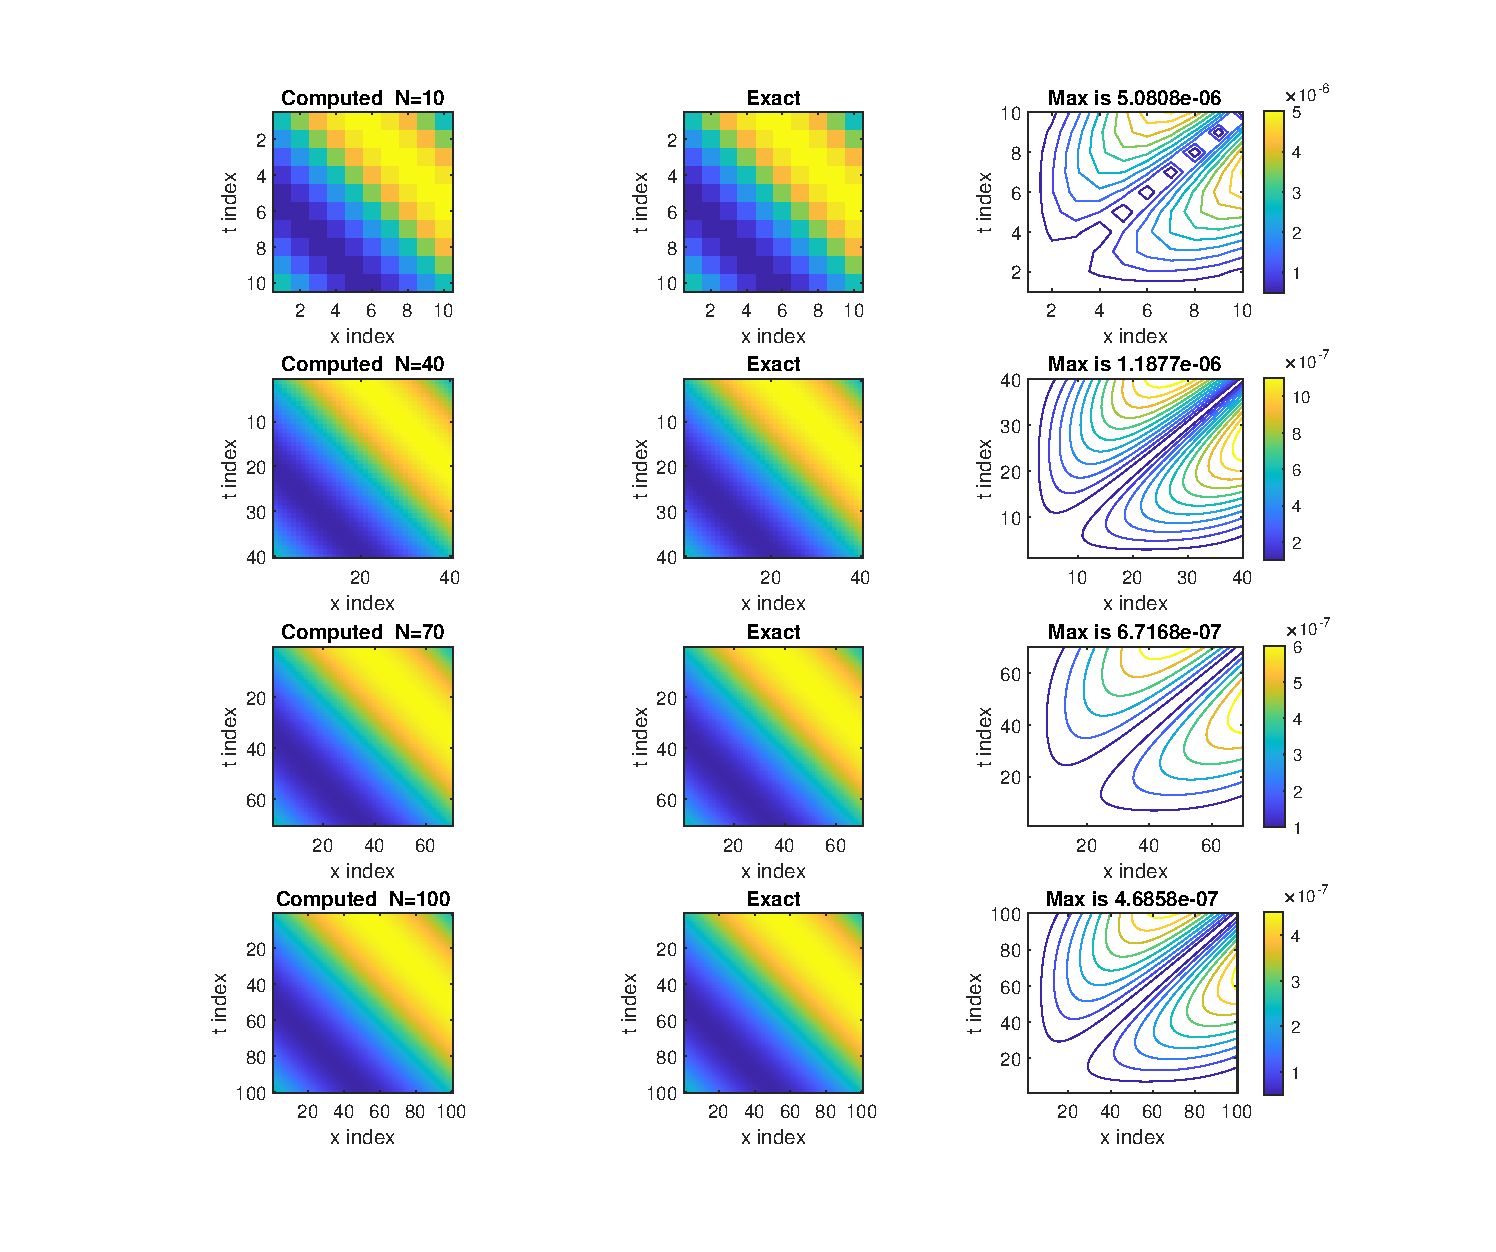
\includegraphics[width=\textwidth]{Fig1.eps}
\caption{Grid‑refinement test for the 1D advection example.
For each grid size $N\in\{10,40,70,100\}$, the normalized intensity images of computed solution, exact solution, and contour plot of absolute error with colorbar are shown.
Each contour subplot displays the maximum absolute error for that resolution in its title.}
\label{fig:1}
\end{figure}

\begin{example}\cite{Chen2021}
Consider the linear advection equation with variable coefficients
\begin{equation}
u_t +  \sin(x)\,u_x + \cos(x)\,u = 0,\quad (x,t)\in[0,1]\times [0,1].
\end{equation}
We impose the initial condition
\[
u(x,0)=1,
\]
together with the boundary condition at $x=0$
\[
u(0,t)=e^{-t}.
\]
The exact solution to this problem is
\[
u(x,t)=\frac{\sin\big(2\arctan\left(e^{-t}\tan(x/2)\right)\big)}{\sin(x)}.
\]
Following equation \eqref{22}, for patch size $s=2$ and indices $i,j\geq 2$, our discrete formulation reads
\[
\frac{1}{h_t}\mathrm{NN}_t\left(
\begin{bmatrix}
F_{(i-1)(j-1)} & F_{(i-1)j}\\
F_{i(j-1)} & F_{ij}
\end{bmatrix}
\right)
+
\sin(x_i)\cdot \frac{1}{h_x}\mathrm{NN}_x\left(
\begin{bmatrix}
F_{(i-1)(j-1)} & F_{(i-1)j}\\
F_{i(j-1)} & F_{ij}
\end{bmatrix}
\right)
+
\cos(x_i)\,F_{ij}
=0.
\]
Rearranging terms isolates the contribution of the grid value $F_{ij}$:
\begin{equation}\label{26}
\left(w_{22}^{[t]}h_x+h_t\sin(x_i){w_{22}^{[x]}}+h_xh_t\cos(x_i)\right)F_{ij}=-\mathcal{R}_{ij},
\end{equation}
where the tail residual term $\mathcal{R}_{ij}$ aggregates all contributions from neighbouring patch entries, including boundary values $F_{1j}$ and initial values $F_{i1}$ for points near the domain edges:
\[
\mathcal{R}_{ij} = h_x\mathrm{NN}_t\left(
\begin{bmatrix}
F_{(i-1)(j-1)} & F_{(i-1)j}\\
F_{i(j-1)} & 0
\end{bmatrix}
\right)
+
\sin(x_i)\cdot h_t\mathrm{NN}_x\left(
\begin{bmatrix}
F_{(i-1)(j-1)} & F_{(i-1)j}\\
F_{i(j-1)} & 0
\end{bmatrix}
\right).
\]
For grid points on the domain boundary or initial line ($i=1$ or $j=1$), we directly set $F_{1j}=e^{-t_j}$ and $F_{i1}=1$ from the prescribed boundary and initial data. Solving equation \eqref{26} along the $t$-direction yields $F_{2j}$ for $j=2,\ldots,N_t$. The remaining grid values are then computed sequentially in the same fashion. Grid refinement tests are performed for $N_x=N_t \in \{10,50,100,500,1000\}$.
Table~\ref{tab:6} summarizes the mean squared error (MSE) for each grid resolution and verifies convergence of the proposed 2-patch neural network scheme. Numerical results for $N_x=N_t=1000$ are illustrated in Figure~\ref{fig:2}.


\end{example}
\begin{figure}[htbp]
\centering
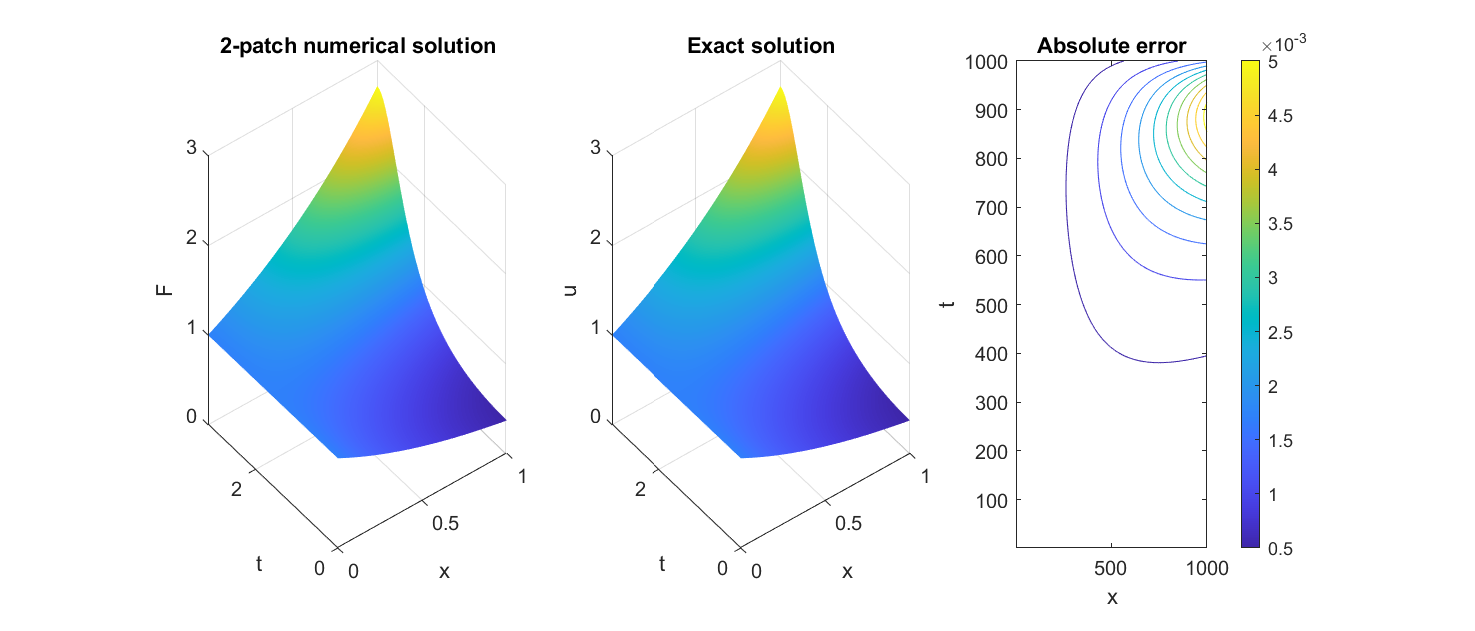
\includegraphics[width=\textwidth]{Fig2.eps}
\caption{Numerical results for the 1D variable-coefficient linear advection problem.
The left panel shows the 2-patch numerical solution, the middle panel presents the exact solution, and the right panel displays the contour plot of absolute error with colorbar.
This result is computed on a grid with $N_x=N_t=1000$.}
\label{fig:2}
\end{figure}
\begin{table}[htbp]
\centering
\caption{Mean squared error (MSE) for grid refinement tests with $N_x=N_t$.}
\begin{tabular}{cccccc}
\toprule
$N_x=N_t$ & 10 & 50 & 100 & 500 & 1000  \\
\midrule
MSE & $2.1676\times 10^{-2}$ & $5.3159\times 10^{-4}$ & $1.2745\times 10^{-4}$ & $4.9418\times 10^{-6}$ & $1.2328\times 10^{-6}$  \\
\bottomrule
\end{tabular}
\label{tab:6}
\end{table}
\section{Deepening 2D NN with Pre-trained NN}\rev{\label{sec:deep}}
Thus far, we have been able to directly train a one-layer linear model without gradient-descent-based methods. The question arises: if we increase the depth of our neural network, how can we formulate the corresponding nonlinear optimization problem that governs this nonlinear setting?

To clarify, we recap the standard approach for deepening a neural network. Let $P$ denote an input patch and $Y$ denote its target output.

Previously, we trained a one-layer linear transform of the form
\[
Z^{[1]}=\langle\boldsymbol{W^{[1]}}, P\rangle + b^{[1]}.
\]
Its nonlinear counterpart can be written as
\[
N^{[1]}(P)=\sigma(Z^{[1]}),
\]
where $\sigma:\mathbb{R}\to \mathbb{R}$ is an activation function (identity, $\tanh$ or sigmoid in our experiments). Adding a second layer gives
\[
Z^{[2]}=\langle\boldsymbol{W^{[2]}}, N^{[1]}(P)\rangle + b^{[2]}.
\]

Gradient-descent-type methods (such as ADAM, SGD, etc.) allow us to iteratively approximate the optimal parameters $b^{[1]},\boldsymbol{W^{[1]}},b^{[2]},\boldsymbol{W^{[2]}}$ simultaneously at each iteration. This renders our earlier gradient root-finding method inapplicable, as the gradient becomes nonlinear.

We seek an alternative strategy that retains our prior direct root‑finding approach via transformation of linear algebraic equations. Under this strategy, we first train $Z^{[1]}$ such that it approximates $Y$, yielding pre‑trained parameters $b^{[1]},\boldsymbol{W}^{[1]}$. We then train
\[
Z^{[2]}=\langle\boldsymbol{W}^{[2]}, N^{[1]}(P)\rangle + b^{[2]}+Z^{[1]}.
\]
In effect, we treat
\[
R=\langle\boldsymbol{W}^{[2]}, N^{[1]}(P)\rangle + b^{[2]}
\]
as a corrector for the pre‑trained model, with the expectation that it improves prediction accuracy. The resulting network is deepened to depth 2 and incorporates the nonlinear activation $\sigma$.

To implement our method for computing partial derivatives, let $\{\boldsymbol{W}^{[x,1]},b^{[x,1]}\}$ and $\{\boldsymbol{W}^{[y,1]},b^{[y,1]}\}$ denote the pre‑trained weights obtained from optimizing the MSE losses \eqref{E11} and \eqref{E12} for derivatives in the $x$ and $y$ directions, respectively. We obtain the second‑layer parameters $\{\boldsymbol{W}^{[x,2]},b^{[x,2]}\}$ and $\{\boldsymbol{W}^{[y,2]},b^{[y,2]}\}$ by optimizing the following MSE loss functions:
\begin{align}
\mathcal{L}_x^{[2]} &= \frac{1}{N}\sum_{F\in\mathbb{S}}\sum_{i,j=n}^{n_x,n_y} \left( \frac{\partial F}{\partial X}\bigg|_{(X_i,Y_j)} - \operatorname{NN}^{[2]}_x(P_{ij}^{[1]})  \right)^{\!2},\label{E27}\\
\mathcal{L}_y^{[2]} &= \frac{1}{N}\sum_{F\in\mathbb{S}}\sum_{i,j=n}^{n_x,n_y} \left( \frac{\partial F}{\partial Y}\bigg|_{(X_i,Y_j)} - \operatorname{NN}^{[2]}_y(P_{ij}^{[1]}) \right)^{\!2},\label{E28}
\end{align}
where
\begin{align}
\operatorname{NN}^{[2]}_x(P_{ij}^{[1]}) &= \langle\boldsymbol{W}^{[x,2]}, P_{x,ij}^{[2]}\rangle + b^{[x,2]}+Z_{x,ij}^{[1]},\\
\operatorname{NN}^{[2]}_y(P_{ij}^{[1]}) &= \langle\boldsymbol{W}^{[y,2]}, P_{y,ij}^{[2]}\rangle + b^{[y,2]}+Z_{y,ij}^{[1]},
\end{align}
and $N_x^{[1]}(P_{ij})$, $N_y^{[1]}(P_{ij})$, $Z_{x,ij}^{[1]}$, and $Z_{y,ij}^{[1]}$ are outputs from the pre‑trained neural network given by
\begin{align}
Z_{\rev{\to},ij}^{[1]} &=\frac{1}{h_{\to}} \left(\langle\boldsymbol{W}^{[\to,1]}, P_{ij}^{[1]}\rangle + b^{[\to,1]}\right),\\
N_{\to,ij}^{[1]} &= \sigma(Z_{\to,ij}^{[1]}).
\end{align}
Let $N_{\to}^{[1]}=(N_{\to,ij}^{[1]})$ denote the corresponding matrix. Then $P_{\to,ij}^{[2]}$ are the $s$-patches obtained from $N_{\to}^{[1]}$, where $\to$ can be $x$ or $y$.

Now, define the corrected target (known data):
\[
\tilde D_{ij} := \left.\frac{\partial F}{\partial X}\right|_{(X_i,Y_j)} - Z_{x,ij}^{[1]}.
\]
The second‑stage MSE loss reads
\[
\mathcal L_x^{[2]}=\frac1N\sum_{F\in\mathbb S}\sum_{i,j\ge n}\Big(\tilde D_{ij}-\langle W^{[x,2]},P_{x,ij}^{[2]}\rangle-b^{[x,2]}\Big)^2.
\]
Set gradients with respect to the unknowns $W^{[x,2]}_{op},b^{[x,2]}$ to zero.
Introduce aggregated summation terms
\[
\begin{aligned}
\widetilde\Theta_{lk,op} &= \sum_{F\in\mathbb S}\sum_{i,j\ge n} \big(P_{x,ij}^{[2]}\big)_{op}\big(P_{x,ij}^{[2]}\big)_{lk},\\
\widetilde\zeta_{lk} &= \sum_{F\in\mathbb S}\sum_{i,j\ge n} \big(P_{x,ij}^{[2]}\big)_{lk},\\
\widetilde\Phi_{lk} &= \sum_{F\in\mathbb S}\sum_{i,j\ge n} \tilde D_{ij}\,\big(P_{x,ij}^{[2]}\big)_{lk}.
\end{aligned}
\]
Using the composite‑index trick for the bias term introduced in Section~\ref{sec:4}, we obtain the linear system analogous to Eq.~\eqref{17}:
\begin{equation}
\sum_{o,p=1}^{s} W^{[x,2]}_{op}\,\widetilde\Theta_{lk,op}
\,+\, b^{[x,2]}\,\widetilde\zeta_{lk}
=\widetilde\Phi_{lk},\quad
lk\in\big\{lk:l,k=1,\dots,s\big\}\cup\big\{s(s+1)\big\}.
\label{eq:17_second_layer}
\end{equation}
The unknown vector is $\mathbf u_2=\big[W^{[x,2]}_{11},\dots,W^{[x,2]}_{ss},\,b^{[x,2]}\big]^T\in\mathbb R^{s^2+1}$, giving $\widetilde A\mathbf u_2=\widetilde{\boldsymbol\Phi}$, solvable by direct linear solvers.
For the $y$-direction, replace $x$ with $y$ and use $N_{y,ij}^{[1]}$, $\tilde D_{ij}^y=\left.\partial F/\partial Y\right|_{ij}-Z_{y,ij}^{[1]}$.

Table \ref{tab:table7} reports the average training MSE obtained for one-layer and two-layer models under data sets of Subsection \ref{subsec431}, with \(h=0.000001\). The two-layer corrector reduces the average training error, and the identity activation produces the lowest MSE among the three considered choices. Sigmoid and $\tanh$ activations give slightly larger training errors compared with the identity case. Table \ref{tab:8} presents the numerical error for the $y$-derivative approximation on the test function $F=\exp(\cos(X^2-Y^2+XY))$ for a range of grid sizes $h$ with sigmoid nonlinearity and $T=0.5$. The two-layer method consistently achieves lower MSE than the one-layer stencil across all examined mesh resolutions. Note that with the identity activation the two-layer model is still a linear operator; its improvement comes from the enlarged effective stencil, since an $s$-patch of first-layer outputs depends on a $(2s-1)\times(2s-1)$ neighbourhood of the original field (a $3\times 3$ neighbourhood for $s=2$).

\begin{table}[htbp]
\centering
\caption{Average training MSE for one-layer and two-layer models with different activation functions.}
\begin{tabular}{cccc}
Model & $\sigma(z)=z$ (identity) & $\sigma(z)=\tanh(z)$ & $\sigma(z)=\text{sigmoid}(z)$ \\
\hline
One-layer & $1.736686\times 10^{-6}$ & $1.736686\times 10^{-6}$ & $1.736686\times 10^{-6}$ \\
Two-layer & $4.523627\times 10^{-7}$ & $6.005541\times 10^{-7}$ & $4.931729\times 10^{-7}$
\end{tabular}
\label{tab:table7}
\end{table}

\begin{table}[htbp]
\centering
\caption{Comparison of MSE for $y$-derivative, one-layer versus two-layer model, test function $F=\exp(\cos(X^2-Y^2+XY))$.}
\begin{tabular}{ccc}
$h$ & $\text{MSE}_y$ (1-layer) & $\text{MSE}_y$ (2-layer) \\
\hline
0.1000 & 5.33719251e-02 & 3.09788164e-02 \\
0.0500 & 1.40022428e-02 & 6.01809198e-03 \\
0.0100 & 5.79167544e-04 & 2.24838304e-04 \\
0.0050 & 1.47743494e-04 & 5.98524716e-05 \\
0.0010 & 7.30650815e-06 & 4.18204181e-06 \\
\end{tabular}
\label{tab:8}
\end{table}
 
\begin{remark}
While the method works for the present examples, our numerical experiments show that deepening the network under this learning philosophy does not produce extreme error reduction for derivative approximation in other training cases.
\end{remark}

\section{Generalizing for 3D NN (Tensors)}\rev{\label{sec:3dnn}}


Let  $F\in\mathbb{R}^{N_x\times N_y\times N_z}$  be a 3D array (a tensor). Typical examples are volumetric data (e.g., CT or MRI scans) and space--time fields $F(t,y,z)$ sampled on a regular grid (An RGB image is also a 3D array).


\subsection{Cubic $s$-Patches}\rev{\label{subsec:cubic}}
Voxel values required for derivative computation are extracted from local cubic patches $P_{abc}$ sampled over the tensor field $F\in\mathbb{R}^{N_x\times N_y\times N_z}$. A stride of 1 is used, so each patch produces one derivative estimate at a grid point.

Boundary points lack the samples required by backward stencils. Constant replication padding is applied: out-of-bounds indices are replaced by the first valid index, enforcing zero derivatives on boundaries.

For target coordinate $(a,b,c)$, define global indices
\[
i_g = a-s+\alpha,\quad j_g = b-s+\beta,\quad k_g = c-s+\gamma,
\]
where local patch indices satisfy $\alpha,\beta,\gamma = 1,2,\dots,s$. The cubic patch $P_{abc}\in\mathbb{R}^{s\times s\times s}$ is defined piecewise:
\begin{equation}
P_{abc}(\alpha,\beta,\gamma)=
\begin{cases}
F_{i_g,j_g,k_g}, & i_g\ge 1,\; j_g\ge 1,\; k_g\ge 1,\\
F_{1,j_g,k_g}, & i_g<1,\; j_g\ge 1,\; k_g\ge 1,\\
F_{i_g,1,k_g}, & i_g\ge 1,\; j_g<1,\; k_g\ge 1,\\
F_{i_g,j_g,1}, & i_g\ge 1,\; j_g\ge 1,\; k_g<1,\\
F_{1,1,k_g}, & i_g<1,\; j_g<1,\; k_g\ge 1,\\
F_{1,j_g,1}, & i_g<1,\; j_g\ge 1,\; k_g<1,\\
F_{i_g,1,1}, & i_g\ge 1,\; j_g<1,\; k_g<1,\\
F_{1,1,1}, & i_g<1,\; j_g<1,\; k_g<1.
\end{cases}
\label{eq:patch_def_3d}
\end{equation}

\paragraph{Example for $s=2$}
In the following, each cubic patch is displayed as two $2\times 2$ slices, $\gamma=1$ (left) and $\gamma=2$ (right); within each slice, rows correspond to $\alpha$ and columns to $\beta$.

Patch $P_{111}$ (corner):
\[
P_{111}=
\begin{bmatrix}
F_{111} & F_{111}\\
F_{111} & F_{111}
\end{bmatrix}
\begin{bmatrix}
F_{111} & F_{111}\\
F_{111} & F_{111}
\end{bmatrix}.
\]
Patch $P_{112}$ (edge):
\[
P_{112}=
\begin{bmatrix}
F_{111} & F_{111}\\
F_{111} & F_{111}
\end{bmatrix}
\begin{bmatrix}
F_{112} & F_{112}\\
F_{112} & F_{112}
\end{bmatrix}.
\]

Patch $P_{121}$ (edge):
\[
P_{121}=
\begin{bmatrix}
F_{111} & F_{121}\\
F_{111} & F_{121}
\end{bmatrix}
\begin{bmatrix}
F_{111} & F_{121}\\
F_{111} & F_{121}
\end{bmatrix}.
\]

Patch $P_{211}$ (edge):
\[
P_{211}=
\begin{bmatrix}
F_{111} & F_{111}\\
F_{211} & F_{211}
\end{bmatrix}
\begin{bmatrix}
F_{111} & F_{111}\\
F_{211} & F_{211}
\end{bmatrix}.
\]

Patch $P_{222}$ (interior point):

\[
P_{222}=
\begin{bmatrix}
F_{111} & F_{121}\\
F_{211} & F_{221}
\end{bmatrix}
\begin{bmatrix}
F_{112} & F_{122}\\
F_{212} & F_{222}
\end{bmatrix}.
\]



Let $\to$ denote one of the directions $x$, $y$, or $z$. We propose the following neural network for computing the derivative in the $\to$ direction on cubic $s$-patches $P_{ijk}$:
\[
D^{[\to]}_{ijk} =\frac{1}{h_{\to}}NN_{\to}^{s\text{-Patch}}(P_{ijk})=\frac{1}{h_{\to}}\left( \langle \boldsymbol{W}^{[\to]}, P_{ijk} \rangle + b^{[\to]}\right),
\]
where $\langle\cdot,\cdot\rangle$ denotes the Frobenius inner product on $\mathbb{R}^{s\times s\times s}$, defined by
\[
\langle A,B\rangle:=\operatorname{sum}(A\odot B):=\sum_{\alpha,\beta,\gamma=1}^{s}a_{\alpha\beta\gamma}b_{\alpha\beta\gamma},
\]
for $A=(a_{\alpha\beta\gamma})\in\mathbb{R}^{s\times s\times s}$ and $B=(b_{\alpha\beta\gamma})\in \mathbb{R}^{s\times s\times s}$.
The loss function is
\[
\mathcal{L}_{\to} = \frac{1}{N}\sum_{F\in\mathbb{S}}\sum_{i,j,k=s}^{n_x,n_y,n_z} \left( \left.\frac{\partial F}{\partial \to}\right|_{(X_i,Y_j,Z_k)} - \frac{1}{h_{\to}}NN_{\to}^{s\text{-Patch}}(P_{ijk}) \right)^{\!2}.
\]

Optimality conditions are obtained by setting gradients of $\mathcal L_{\to}$ with respect to tensor entries $W^{[\to]}_{\alpha\beta\gamma}$ and scalar bias $b^{[\to]}$ to zero. Define the aggregated summation quantities
\begin{align}
\Theta_{\alpha'\beta'\gamma',\alpha\beta\gamma}
=&\sum_{F\in\mathbb S}\sum_{i,j,k\ge s}
(P_{ijk})_{\alpha\beta\gamma}\,(P_{ijk})_{\alpha'\beta'\gamma'}, \label{35E} \\
\zeta_{\alpha'\beta'\gamma'}
=&\sum_{F\in\mathbb S}\sum_{i,j,k\ge s}
(P_{ijk})_{\alpha'\beta'\gamma'},\\
\Phi_{\alpha'\beta'\gamma'}
=& h_{\to}\sum_{F\in\mathbb S}\sum_{i,j,k\ge s}
\left.\frac{\partial F}{\partial\to}\right|_{(X_i,Y_j,Z_k)}
\,(P_{ijk})_{\alpha'\beta'\gamma'}. \label{37E}
 \end{align}
This yields the linear algebraic system
\[
\sum_{\alpha,\beta,\gamma=1}^{s} w^{[\to]}_{\alpha\beta\gamma}\,\Theta_{\alpha'\beta'\gamma',\alpha\beta\gamma}
+ b^{[\to]}\,\zeta_{\alpha'\beta'\gamma'}
=\Phi_{\alpha'\beta'\gamma'},
\]
where the indices satisfy
\[
(\alpha',\beta',\gamma') \in \{1,\dots,s\}^3 \cup \{(s,s,s+1)\}.
\]
The composite index $(s,s,s+1)$ corresponds to the bias equation, with associated aggregated quantities 
\begin{align}
 \Theta_{ss(s+1),\,\alpha\beta\gamma} &= \sum_{F\in\mathbb S}\sum_{\substack{i,j,k\ge s}} \big(P_{ijk}\big)_{\alpha\beta\gamma},\label{38E} \\
 \zeta_{ss(s+1)} &= \sum_{F\in\mathbb S}\sum_{\substack{i,j,k\ge s}} 1, \\
 \Phi_{ss(s+1)} &= h_{\to}\sum_{F\in\mathbb S}\sum_{\substack{i,j,k\ge s}} \left.\frac{\partial F}{\partial \to}\right|_{(X_i,Y_j,Z_k)}.\label{40E}
 \end{align}
  Equations \eqref{38E}--\eqref{40E} can be recovered from Equations  \eqref{35E}--\eqref{37E} by imposing the augmented entry $(P_{ijk})_{ss(s+1)}=1.$
 
For $(\alpha',\beta',\gamma') \in \{1,\dots,s\}^3$, the equations arise from zeroing gradients with respect to tensor entries $W^{[\to]}_{\alpha'\beta'\gamma'}$;
for the special index $(s,s,s+1)$, the equation originates from setting $\nabla_{b^{[\to]}}\mathcal{L}_{\to}=0$.



The unknown vector
\[
\boldsymbol u^{[\to]}=\big[w^{[\to]}_{111},w^{[\to]}_{112},\dots,w^{[\to]}_{sss},\; b^{[\to]}\big]^T\in\mathbb R^{s^3+1}
\]
satisfies $\boldsymbol A^{[\to]}\boldsymbol u^{[\to]}=\boldsymbol\Phi^{[\to]}$, which can be solved via direct linear solvers.



Following Subsection \ref{subsec431}, we construct training data for the  derivative approximation  using the following functions:
\begin{align*}
&cX^s,\quad \quad  cY^t,\quad \quad  cZ^u,\quad \quad   c,\quad 30\times 3+6\ \text{data} \\
&cX^s Y^t Z^u,\quad \quad X^s + cY^t+Z^u, \quad \quad cX^s + Y^t+Z^u, \quad \quad X^s + Y^t+cZ^u,\quad 750\times 4\ \text{data}\\
&\sin(cX^s Y^t Z^u), 750\ \text{data} \\% \quad  \sin(cX^s + Y^t),\quad  \sin(X^s + zY^t),
&\cos(cX^s Y^t Z^u), 750\ \text{data} \\ % \quad \cos(cX^s + Y^t),\quad \cos(X^s + zY^t),
&\exp(cX^s Y^t Z^u), 750\ \text{data} %\quad  \exp(cX^s + Y^t),\quad  \exp(X^s + cY^t),
\end{align*}
where
$s,t,u \in \{1,\dots,5\}$ and $ c\in \{\pm1,\dots,\pm3\}.$ This set yields a total of $5346$ training samples.


\begin{table}[ht]
\centering
\caption{Average training MSE for the $x$-, $y$-, and $z$-direction derivative approximations using cubic $s$-patches, with $N=5$, $T=0.00005$ and $s=2$.}
\begin{tabular}{cccc}
\hline
Direction & $x$ & $y$ & $z$ \\
\hline
MSE & $3.508474\times 10^{-11}$ & $3.508474\times 10^{-11}$ & $3.243698\times 10^{-11}$ \\
\hline
\end{tabular}
\label{tab:9}
\end{table}

Table \ref{tab:9} reports the average training MSE of our cubic $s$-patch network for the three spatial directions, obtained for parameters $N=5$, $T=0.00005$, and patch size $s=2$. 
As an example, the learned weight tensor and bias for the $x$-direction are
\[
\boldsymbol{W}^{[x]}=
\begin{pmatrix}
-0.357792060386 & -0.654036140366 \\
-0.654036144784 &  1.665863225142
\end{pmatrix}
\begin{pmatrix}
  1.288510866291    & -1.276673224973 \\
-0.276681804994 &      0.264845284057
\end{pmatrix},\]
\[
b^{[x]} = 1.48525005253\times 10^{-11}.
\]

\begin{remark}
The solution computed via the backslash operator $\boldsymbol{u}^{[\to]}=\boldsymbol{A}^{[\to]} \backslash \boldsymbol{\Phi}^{[\to]}$ in MATLAB is only one particular member of the solution family: for a rank-deficient Gram matrix $\boldsymbol{A}^{[\to]}$, backslash returns a basic solution, which in general is not the minimum-norm solution (the latter is given by \texttt{lsqminnorm} or \texttt{pinv}). While this approach yields low static derivative fitting error, it provides no direct access to the remaining degrees of freedom in the solution family and offers no transparent way to enforce the recurrence stability condition,  a problem we investigate subsequently. To overcome this limitation, we instead perform Gaussian elimination via elementary row operations on the augmented matrix $[\boldsymbol{A}^{[\to]} \mid \boldsymbol{\Phi}^{[\to]}]$ to obtain its reduced row echelon form. This explicit algebraic representation separates pivot variables from free parameters, parameterizing the entire affine set of consistent stencils and enabling us to search within this family for weights that satisfy both the discrete derivative consistency and the stability requirement for marching in numerical methods we later investigate.
\end{remark}
\section{Solving PDEs with Three Independent Variables}\rev{\label{sec:pde3d}}
Consider PDEs of the form
\begin{equation}
G\left(X,Y,Z,F,\frac{\partial F}{\partial X},\frac{\partial F}{\partial Y},\frac{\partial F}{\partial Z}\right)=0,
\label{eq:3d-pde-general}
\end{equation}
where $G:\mathbb{R}^7\to\mathbb{R}$ is a continuous real-valued function. This general class covers a wide range of first-order linear, quasilinear and fully nonlinear PDEs including three-dimensional linear advection \cite{Benson2025,Peters2007}, Hamilton--Jacobi, and eikonal equations \cite{Kao2005}, which arise in atmospheric transport, geometric optics and wave propagation problems. The PDE is supplemented by boundary conditions defined on the three coordinate planes:
\begin{equation}
F(0,Y,Z)=\Theta_1(Y,Z),\quad
F(X,0,Z)=\Theta_2(X,Z),\quad
F(X,Y,0)=\Theta_3(X,Y),
\end{equation}
where $\Theta_1,\Theta_2,\Theta_3$ are given continuous boundary functions.

We discretize the domain on a uniform Cartesian mesh with grid spacings $h_x,h_y,h_z$. The grid coordinates read
\[
X_i = (i-1) h_x,\quad Y_j = (j-1) h_y,\quad Z_k = (k-1) h_z,
\]
for integer indices $i,j,k\ge 1$, so that the index $1$ corresponds to the coordinate planes. At each grid point $(i,j,k)$ we extract a cubic backward $s$-patch $P_{ijk}\in\mathbb{R}^{s\times s\times s}$ as defined in Subsection \rev{\ref{subsec:cubic}}. Boundary out-of-range indices are handled by constant-replication padding.

Using the pre-trained three-dimensional $s$-patch derivative operators from Section \rev{\ref{sec:3dnn}}, the continuous partial derivatives are approximated as
\[
\left.\frac{\partial F}{\partial X}\right|_{(X_i,Y_j,Z_k)}
\approx \frac{1}{h_x}\, \mathrm{NN}_x^{s\text{-patch}}(P_{ijk}),
\]
\[
\left.\frac{\partial F}{\partial Y}\right|_{(X_i,Y_j,Z_k)}
\approx \frac{1}{h_y}\, \mathrm{NN}_y^{s\text{-patch}}(P_{ijk}),
\]
\[
\left.\frac{\partial F}{\partial Z}\right|_{(X_i,Y_j,Z_k)}
\approx \frac{1}{h_z}\, \mathrm{NN}_z^{s\text{-patch}}(P_{ijk}),
\]
with
\[
\mathrm{NN}_{\to}^{s\text{-patch}}(P_{ijk})
=\bigl\langle w^{[\to]}, P_{ijk}\bigr\rangle + b^{[\to]},
\]
where $\to\in\{x,y,z\}$, $\langle\cdot,\cdot\rangle$ denotes the three-dimensional Frobenius inner product for tensors, and $w^{[\to]},b^{[\to]}$ are the pre‑learned tensor weight and scalar bias obtained by solving the linear system described in Section \rev{\ref{sec:3dnn}}.

Substituting these data‑informed derivative approximations into the governing PDE \eqref{eq:3d-pde-general} yields a discrete nonlinear algebraic equation at each interior grid point:
\begin{equation}
G\left(X_i,Y_j,Z_k,\;F_{ijk},\;
\frac{1}{h_x}\mathrm{NN}_x^{s\text{-patch}}(P_{ijk}),\;
\frac{1}{h_y}\mathrm{NN}_y^{s\text{-patch}}(P_{ijk}),\;
\frac{1}{h_z}\mathrm{NN}_z^{s\text{-patch}}(P_{ijk})
\right)=0.
\label{eq:discrete-3d-pde}
\end{equation}

For patch size $s$, the marching solution procedure starts from the given boundary data on the three planes $i=1$, $j=1$, $k=1$:
\[
F_{1jk}=\Theta_1(Y_j,Z_k),\quad
F_{i1k}=\Theta_2(X_i,Z_k),\quad
F_{ij1}=\Theta_3(X_i,Y_j).
\]
These boundary values fill the required entries inside the cubic backward patches for points near domain boundaries, applying the padding rules from Subsection \rev{\ref{subsec:cubic}}.

We then march over interior indices $i,j,k \ge s$. For each target grid point $(i,j,k)$, the patch $P_{ijk}$ contains known field values from previously computed neighbouring grid entries plus the single unknown grid value $F_{ijk}$. Expanding the inner‑product form of the $s$-patch operator separates terms involving the unknown $F_{ijk}$ from all other known patch entries:
\[
\mathrm{NN}_{\to}^{s\text{-patch}}(P_{ijk})
= w_{sss}^{[\to]}\,F_{ijk}
+ \sum_{\substack{\alpha,\beta,\gamma=1\\(\alpha,\beta,\gamma)\ne(s,s,s)}}^s w_{\alpha\beta\gamma}^{[\to]}\,(P_{ijk})_{\alpha\beta\gamma}
+ b^{[\to]}.
\]
Define the known residual contributions
\[
\mathcal{R}_{ijk}^{[\to]}
= \sum_{\substack{\alpha,\beta,\gamma=1\\(\alpha,\beta,\gamma)\ne(s,s,s)}}^s w_{\alpha\beta\gamma}^{[\to]}\,(P_{ijk})_{\alpha\beta\gamma}
+ b^{[\to]}.
\]
Then each derivative approximation becomes
\[
\frac{1}{h_\to}\mathrm{NN}_{\to}^{s\text{-patch}}(P_{ijk})
=\frac{w_{sss}^{[\to]}}{h_\to} F_{ijk}
+\frac{1}{h_\to}\mathcal{R}_{ijk}^{[\to]}.
\]
Inserting into \eqref{eq:discrete-3d-pde} gives
\begin{equation}\label{44}
G\biggl(X_i,Y_j,Z_k,\;F_{ijk},\;
\frac{w_{sss}^{[x]}}{h_x}F_{ijk}+\frac{1}{h_x}\mathcal{R}_{ijk}^{[x]},\;
\frac{w_{sss}^{[y]}}{h_y}F_{ijk}+\frac{1}{h_y}\mathcal{R}_{ijk}^{[y]},\;
\frac{w_{sss}^{[z]}}{h_z}F_{ijk}+\frac{1}{h_z}\mathcal{R}_{ijk}^{[z]}
\biggr)=0.
\end{equation}
This is a scalar nonlinear equation for the single unknown $F_{ijk}$. It can be solved locally for each grid point using a root‑finding algorithm. Once $F_{ijk}$ is computed, it becomes available as known data for subsequent patches in the marching sweep.

\begin{example}{\bf (Uniform advection with constant velocity)}
Consider the linear transport equation
\begin{equation}\label{45}
\frac{\partial F}{\partial t}+\frac{\partial F}{\partial y}+\frac{\partial F}{\partial z}=0,
\end{equation}
which describes pure advection in the $(y,z)$‑plane with constant unit velocity field $(1,1)$. The problem is equipped with the Gaussian initial condition
\[
F(0,y,z)=\exp\big(-y^2-z^2\big),
\]
centered at the origin of the spatial domain at $t=0$.
The corresponding exact solution is given by
\[
F(t,y,z)=\exp\Big(-\big((y-t)^2+(z-t)^2\big)\Big).
\]
This solution represents a Gaussian blob that translates uniformly with velocity $(1,1)$ without deformation, diffusion, or amplitude decay over time. For boundary reference, the solution evaluated along the axes yields
\[
F(t,0,z)=\exp\big(-t^2-(z-t)^2\big),\qquad
F(t,y,0)=\exp\big(-(y-t)^2-t^2\big).
\]
This canonical benchmark solution is widely adopted for validating numerical advection schemes, as it provides an exact reference for shape‑preserving translational transport \cite{leveque2002finite}.
\end{example}

In this example, the time variable $t$ plays the role of the first coordinate $X$ in \eqref{eq:3d-pde-general}, i.e., $(X,Y,Z)=(t,y,z)$; accordingly, $h_x$ and $\boldsymbol{W}^{[x]}$ below refer to the $t$-direction.

For this linear advection example, substituting the $s$-patch derivative approximations yields a linear algebraic equation for $F_{ijk}$, which can be solved directly without iterative root‑finding. Grid‑refinement tests can be performed by varying $h_t,h_y,h_z$ and measuring MSE against the exact Gaussian blob solution, verifying convergence of the three‑dimensional $s$-patch marching scheme.

Applying \eqref{44} to equation \eqref{45}, we get 
\begin{equation}
\left(\frac{w_{sss}^{[x]}}{h_x}+
\frac{w_{sss}^{[y]}}{h_y}+
\frac{w_{sss}^{[z]}}{h_z}\right)F_{ijk}+\frac{1}{h_x}\mathcal{R}_{ijk}^{[x]}+\frac{1}{h_y}\mathcal{R}_{ijk}^{[y]}+\frac{1}{h_z}\mathcal{R}_{ijk}^{[z]}=0.
\end{equation}
For uniform grid spacing $h_x=h_y=h_z$, this simplifies to the explicit marching update
\begin{equation}
F_{ijk}=-\frac{\mathcal{R}_{ijk}^{[x]}+\mathcal{R}_{ijk}^{[y]}+\mathcal{R}_{ijk}^{[z]}}{w_{sss}^{[x]}+w_{sss}^{[y]}+w_{sss}^{[z]}}.
\label{eq:marching-update-uniform}
\end{equation}
Equation \eqref{eq:marching-update-uniform} shows clearly that the central coefficients $w_{sss}^{[x]},w_{sss}^{[y]},w_{sss}^{[z]}$ form the denominator of the marching formula. Degeneracy occurs when this sum vanishes, which renders the update undefined.

We first tested stencils obtained purely from derivative fitting on training data. Those fitted weight tensors satisfy the consistency equations, but they often produce unstable marching schemes. The source of instability was traced to spurious cross-coupling terms: grid points shared across two or three directional residuals accumulate error in the combined update. To remove this interference, we introduced four linear cancellation constraints for these shared nodes:
\begin{align}
w_{111}^{[x]} + w_{111}^{[y]} + w_{111}^{[z]} &= 0,\label{E49} \\
w_{121}^{[x]} + w_{121}^{[y]} + w_{121}^{[z]} &= 0,\\
w_{112}^{[x]} + w_{112}^{[y]} + w_{112}^{[z]} &= 0,\\
w_{211}^{[x]} + w_{211}^{[y]} + w_{211}^{[z]} &= 0.\label{E52}
\end{align}
These constraints enforce exact cancellation of the combined contribution from overlapping grid nodes that appear simultaneously in the residual of multiple directional derivative approximations. With these structural constraints active, the solution manifold of the weight tensors is restricted, and the feasible set for the central coefficients $w_{222}^{[x]},w_{222}^{[y]},w_{222}^{[z]}$ (for $s=2$) becomes tightly bounded. Numerical experiments reveal a limited feasible interval for their total sum $S_{\text{central}}=w_{222}^{[x]}+w_{222}^{[y]}+w_{222}^{[z]}$. When $S_{\text{central}}$ was too small, for example $1$ or $2$, the only consistent solution forced one directional weight tensor to vanish, yielding a degenerate, unusable stencil. A non-degenerate consistent family first appears at $S_{\text{central}}=3$. Inside this family, the central weights can be redistributed unequally among directions while keeping their sum fixed at $3$. For instance, the choice $w_{222}^{[x]}=2$, $w_{222}^{[y]}=0.5$, $w_{222}^{[z]}=0.5$ gives a consistent and stable scheme. If we increase the total sum beyond $3.5$, the system again becomes inconsistent, and the solver collapses one directional tensor to zero.

This observation demonstrates that the four cancellation constraints impose an intrinsic compatibility bound on the central coefficients. The symmetric case $w_{222}^{[x]}=w_{222}^{[y]}=w_{222}^{[z]}=1$ is just one special point on the feasible manifold, not the only valid choice. By adjusting the distribution of the fixed total weight $3$ among the three central coefficients, we obtain a continuous family of stencils with different amplification factors, while preserving derivative consistency and cross-term cancellation. This family provides a practical tuning space to select stable schemes with tailored dissipation and dispersion properties.

To apply the structural constraints \eqref{E49}--\eqref{E52}, we append them to the global linear system of discrete consistency equations. We assemble the block-diagonal matrix $\boldsymbol{A}_{\text{big}}=\operatorname{blkdiag}(\boldsymbol{A}^{[x]},\boldsymbol{A}^{[y]},\boldsymbol{A}^{[z]})$ and the stacked right-hand side $\boldsymbol{\Phi}_{\text{big}}=[\boldsymbol{\Phi}^{[x]};\boldsymbol{\Phi}^{[y]};\boldsymbol{\Phi}^{[z]}]$, forming the initial augmented matrix $[\boldsymbol{A}_{\text{big}}\mid \boldsymbol{\Phi}_{\text{big}}]$. The four cancellation constraints are added as additional rows to this augmented system. The reduced row echelon form of the extended matrix identifies pivot unknowns and free parameters. To construct a valid particular solution, we assign values to the free variables and recover all pivot variables by back-substitution; this procedure avoids the inadmissible singular branch where the denominator vanishes.
As an illustration, the weight coefficients for one stable and feasible member of this stencil family are given below:
\[
w^{[x]}=
\begin{bmatrix}
   -0.1000  &  1.1000\\
    0.1000  & -1.1000
\end{bmatrix}
\begin{bmatrix}
    0.0000  & -1.0000\\
   -1.0000  &  2.0000
\end{bmatrix},\qquad
b^{[x]} = 5.1279\times 10^{-12},
\]
\[
w^{[y]}=
\begin{bmatrix}
    0.1000 &  -0.6000\\
    0.4000  &  0.1000
\end{bmatrix}
\begin{bmatrix}
   -0.5000     &    0.0000\\
         0.0000   & 0.5000
\end{bmatrix},\qquad
b^{[y]} = 1.8409\times 10^{-11},
\]
\[
w^{[z]}=
\begin{bmatrix}
    0.0000 &  -0.5000\\
   -0.5000   &     0.0000
\end{bmatrix}
\begin{bmatrix}
    0.5000    &    0.0000\\
        0.0000      & 0.5000
\end{bmatrix},\qquad
b^{[z]} = 1.8409\times 10^{-11}.
\]
The stability of this member can be explained directly. Adding the three weight tensors gives the combined stencil that enters \eqref{eq:marching-update-uniform}:
\[
w^{[x]}+w^{[y]}+w^{[z]}=
\begin{bmatrix}
0 & 0\\
0 & -1
\end{bmatrix}
\begin{bmatrix}
0 & -1\\
-1 & 3
\end{bmatrix}.
\]
With the biases neglected, the marching update \eqref{eq:marching-update-uniform} therefore reduces to
\[
F_{ijk}=\tfrac13\big(F_{i-1,j,k}+F_{i,j-1,k}+F_{i,j,k-1}\big),
\]
which is the classical first-order upwind discretization of \eqref{45} with $h_t=h_y=h_z$. Since $F_{ijk}$ is a convex combination of previously computed values, the scheme satisfies a discrete maximum principle, $\min F\le F_{ijk}\le \max F$, and is therefore stable. The cancellation constraints \eqref{E49}--\eqref{E52} thus steer the learned stencils towards a monotone combined scheme. Each individual tensor is still a consistent first-order derivative stencil, but the stencils are not unique, and only their sum determines the marching update.

This stencil is tested on the uniform advection benchmark. Figure \ref{fig:3} shows numerical results, exact solutions, and pointwise errors at three successive time instants.

\begin{figure}[htbp]
\centering
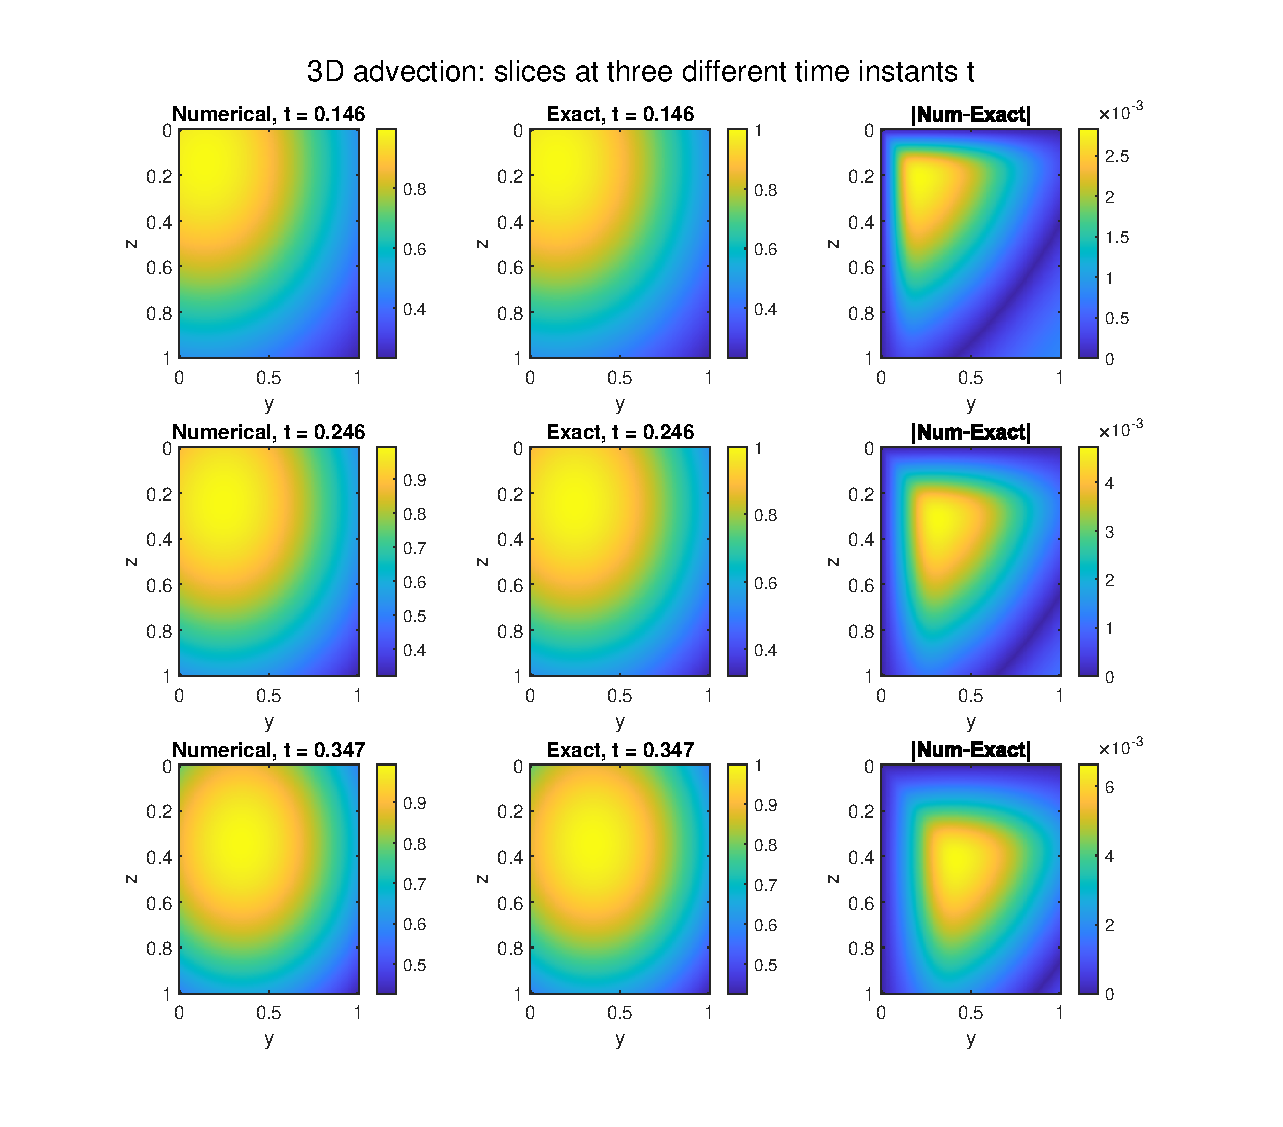
\includegraphics[width=\textwidth]{Fig3.eps}
\caption{3D advection test: numerical solution, exact solution and absolute error $|\text{Num}-\text{Exact}|$ at $t=0.146$, $0.246$, $0.347$. The scheme maintains low error as the Gaussian blob translates.}
\label{fig:3}
\end{figure}

Figure \ref{fig:4} visualises the advection of the Gaussian blob over the time interval $t\in[0,1]$. The stacked $y$--$z$ slices clearly reveal the transport direction captured by the proposed numerical scheme.

\begin{figure}[htbp]
\centering
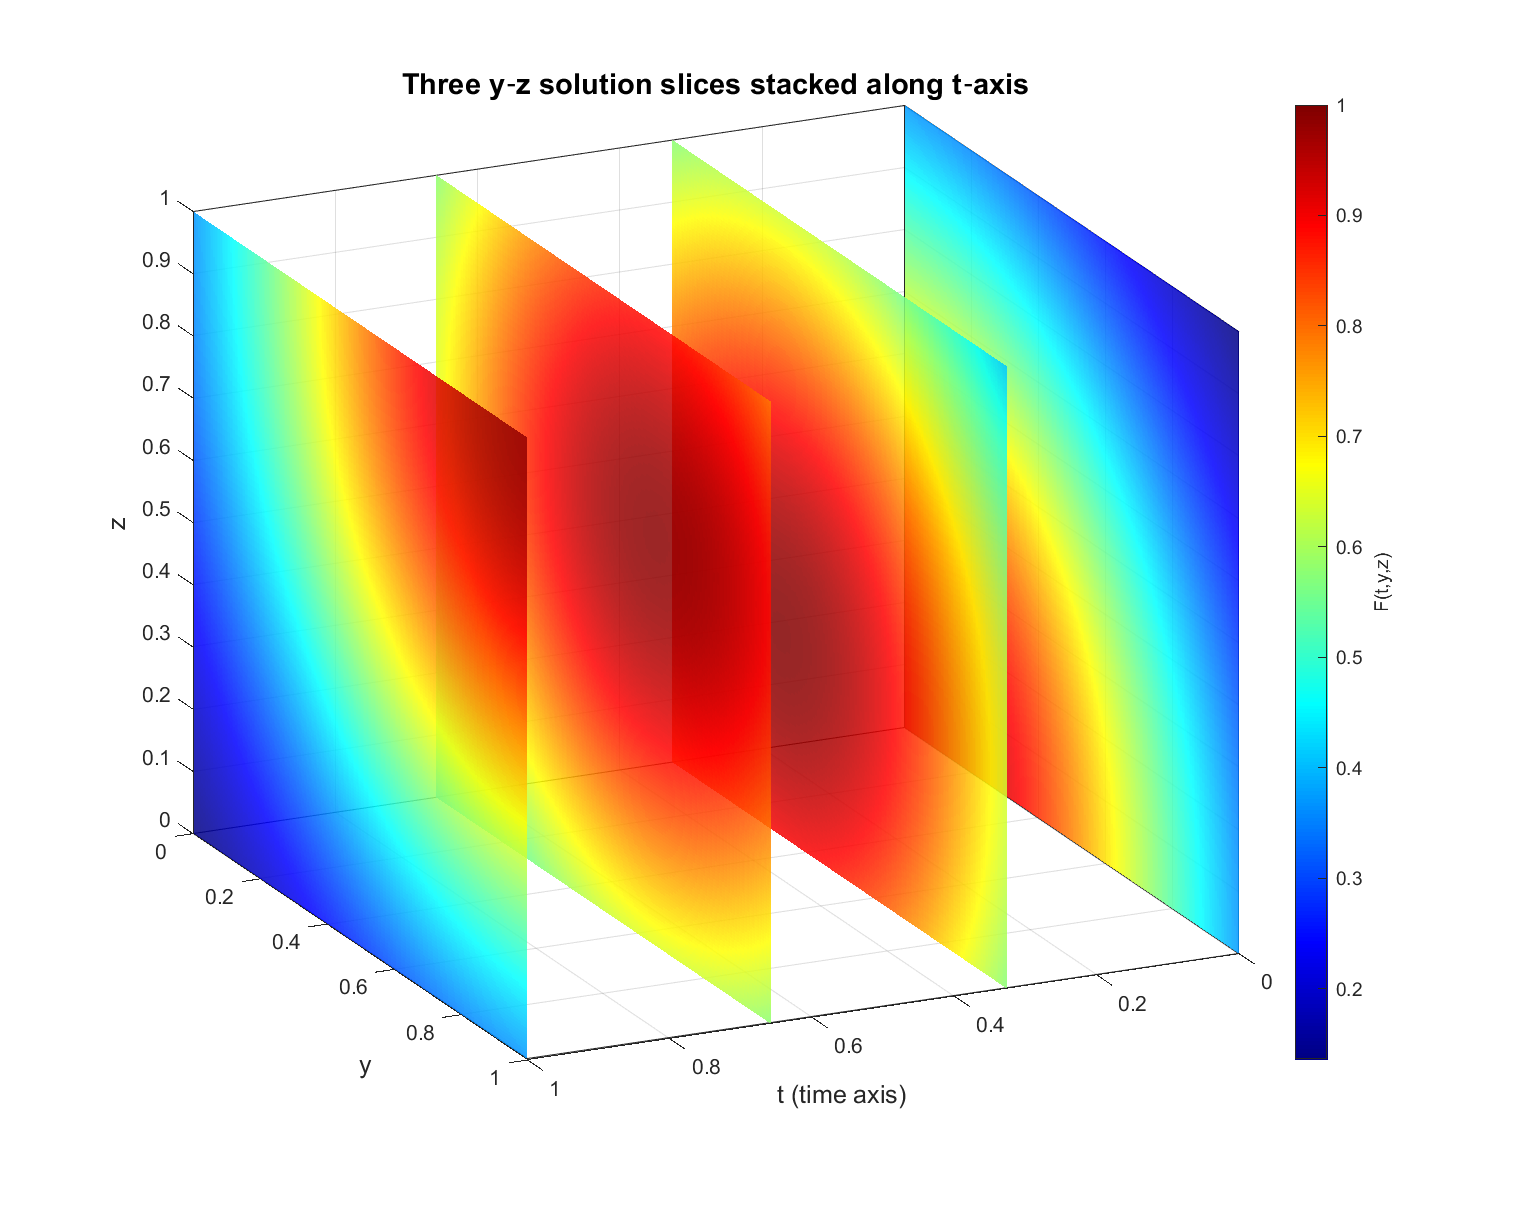
\includegraphics[width=0.9\textwidth]{Fig4.eps}
\caption{Stacked $y$--$z$ slices of the transported Gaussian blob over $t\in[0,1]$, illustrating the advection direction computed by the proposed method.}
\label{fig:4}
\end{figure}

\section{Conclusion}\rev{\label{sec:conclusion}}

This work presented a patch‑based neural‑network framework for data‑informed spatial derivative approximation, which departs from conventional finite‑difference approaches where stencil weights are manually derived. The framework was developed for two‑dimensional matrix fields and further generalized to three‑dimensional tensor data. Backward local patches with constant replication padding were adopted to treat boundary points. Network weights for the single‑layer model were computed by solving linear systems, and the learned derivative operators were integrated into a marching algorithm to solve first‑order partial differential equations. Numerical experiments demonstrated first‑order convergence for derivative approximations, stable PDE solutions in both two and three dimensions, and limited accuracy gains from a two‑layer corrector extension. Structural constraints were introduced to stabilize learned three‑dimensional stencils during PDE marching computations.

The one‑layer formulation in this work leverages direct linear‑system solution for parameter optimization, locating optimal weights without iterative gradient‑descent‑type algorithms such as Adam. In our numerical tests, standard gradient‑based optimizers struggle to converge toward these optimal solutions. This raises an open research question: can analogous direct non‑gradient optimization strategies be constructed for two‑layer or deeper network architectures, to locate optimal parameters without gradient descent? Such capability would represent a meaningful breakthrough for neural‑network training. In the present study, direct solution is feasible because patch‑based formulations keep the total number of trainable parameters low. This points toward a broad, promising research avenue for exploring alternative non‑gradient optimization schemes, as an alternative to the gradient‑based methods that underpin most modern deep‑learning developments. While gradient‑based approaches remain highly successful, there remains scope for advancing alternative learning paradigms. In this paper, we attempted one such strategy: pre‑training the first layer, then solving directly for second‑layer correction weights. Only modest accuracy improvements were achieved with this approach. By contrast, full joint gradient‑descent training of all weights across multiple layers can substantially alter the attained optimal point. Our experiments suggest this joint strategy performs poorly for the single‑layer setting, yet it may remain among the most viable practical options for deep networks.

A second direction for future work follows from the observation that partial derivatives are central to feature and edge detection tasks. The patch‑based methodology developed in this paper could be adapted directly for edge‑detection applications, which constitutes one of our planned next developments. 




\newpage
\section*{Data Availability}
The implementations of the proposed method, including the scripts that generate the training data and reproduce all tables and figures of this paper, are publicly available at https://github.com/USERNAME/REPOSITORY. All training and test data are generated by these scripts from the analytical functions described in the paper; no external datasets were used.

\section*{Conflict of Interest Declaration}
The authors declare that there are no conflicts of interest regarding the publication of this paper. There is no financial or non-financial relationship with any organization or individual that could influence the results and conclusions presented in this study.


\section*{Funding}
The described research originates from the project Research of Excellence on Digital Technologies and Wellbeing CZ.02.01.01/00/22\_008/0004583 which is co-financed by the European Union.
The article has been produced with the financial support of the European Union under the REFRESH – Research Excellence For REgion Sustainability and High-tech Industries project number CZ.10.03.01/00/22\_003/0000048 via the Operational Programme Just Transition.

\begin{thebibliography}{99}


\bibitem{xavier_glorot}
Glorot, X., Bengio, Y.: Understanding the difficulty of training deep feedforward neural networks. In: Proceedings of the 13th International Conference on Artificial Intelligence and Statistics (AISTATS), Proceedings of Machine Learning Research, vol.~9, pp.~249--256 (2010)

%% NOTE: this reference could not be verified online; please check authors, title, volume and pages.
\bibitem{heavy_init}
Cho, Y., Choi, J.: Heavy-tailed weight initialization for deep neural networks. IEEE Access \textbf{9}, 126714--126724 (2021)

\bibitem{kingma2014adam}
Kingma, D.P., Ba, J.: Adam: A method for stochastic optimization. arXiv preprint arXiv:1412.6980 (2014)

\bibitem{Cortes1995}
Cortes, C., Vapnik, V.: Support-vector networks. Machine Learning \textbf{20}(3), 273--297 (1995)

\bibitem{Rumelhart1986}
Rumelhart, D.E., Hinton, G.E., Williams, R.J.: Learning representations by back-propagating errors. Nature \textbf{323}, 533--536 (1986)

\bibitem{Lecun1998}
LeCun, Y., Bottou, L., Bengio, Y., Haffner, P.: Gradient-based learning applied to document recognition. Proceedings of the IEEE \textbf{86}(11), 2278--2324 (1998)

\bibitem{Krizhevsky2012}
Krizhevsky, A., Sutskever, I., Hinton, G.E.: ImageNet classification with deep convolutional neural networks. In: Advances in Neural Information Processing Systems 25 (NIPS 2012), pp.~1097--1105 (2012)

\bibitem{Li2023}
Li, G.: Artificial optical synaptic devices with ultra-low power consumption. Light: Science \& Applications \textbf{12}, 24 (2023)

\bibitem{Beyeler2013}
Beyeler, M., Dutt, N.D., Krichmar, J.L.: Categorization and decision-making in a neurobiologically plausible spiking network using a STDP-like learning rule. Neural Networks \textbf{48}, 109--124 (2013)

\bibitem{Song2024}
Song, A., Kottapalli, S.N.M., Goyal, R., Sch\"{o}lkopf, B., Fischer, P.: Low-power scalable multilayer optoelectronic neural networks enabled with incoherent light. Nature Communications \textbf{15}, 10692 (2024)

\bibitem{raissi2019physics}
Raissi, M., Perdikaris, P., Karniadakis, G.E.: Physics-informed neural networks: A deep learning framework for solving forward and inverse problems involving nonlinear partial differential equations. Journal of Computational Physics \textbf{378}, 686--707 (2019)

\bibitem{lagaris1998artificial}
Lagaris, I.E., Likas, A., Fotiadis, D.I.: Artificial neural networks for solving ordinary and partial differential equations. IEEE Transactions on Neural Networks \textbf{9}(5), 987--1000 (1998)

\bibitem{aarts2001neural}
Aarts, L.P., van der Veer, P.: Neural network method for solving partial differential equations. Neural Processing Letters \textbf{14}, 261--271 (2001)

\bibitem{kumar2011multilayer}
Kumar, M., Yadav, N.: Multilayer perceptrons and radial basis function neural network methods for the solution of differential equations: A survey. Computers \& Mathematics with Applications \textbf{62}(10), 3796--3811 (2011)

\bibitem{shiri2022adaptive}
Shiri, B., Kong, H., Wu, G.-C., Luo, C.: Adaptive learning neural network method for solving time-fractional diffusion equations. Neural Computation \textbf{34}(4), 971--990 (2022)

\bibitem{Ryu2025}
Ryu, J., Park, S., Hwang, H.J.: A physics-informed neural network framework for solving PDEs on point clouds via surface reconstruction. Neural Networks \textbf{192}, 107928 (2025)

\bibitem{Yu2026}
Yu, T., Qiu, J., Yang, J., Oseledets, I.: Sinc Kolmogorov--Arnold network and its application for solving PDEs with singularities. Neural Networks \textbf{202}, 109033 (2026)

\bibitem{cuomo2022review}
Cuomo, S., Schiano Di Cola, V., Giampaolo, F., Rozza, G., Raissi, M., Piccialli, F.: Scientific machine learning through physics-informed neural networks: Where we are and what's next. Journal of Scientific Computing \textbf{92}(3), 88 (2022)

\bibitem{fornberg1988generation}
Fornberg, B.: Generation of finite difference formulas on arbitrarily spaced grids. Mathematics of Computation \textbf{51}(184), 699--706 (1988)

\bibitem{barsinai2019learning}
Bar-Sinai, Y., Hoyer, S., Hickey, J., Brenner, M.P.: Learning data-driven discretizations for partial differential equations. Proceedings of the National Academy of Sciences \textbf{116}(31), 15344--15349 (2019)

\bibitem{long2018pdenet}
Long, Z., Lu, Y., Ma, X., Dong, B.: PDE-Net: Learning PDEs from data. In: Proceedings of the 35th International Conference on Machine Learning (ICML), Proceedings of Machine Learning Research, vol.~80, pp.~3208--3216 (2018)

\bibitem{kochkov2021machine}
Kochkov, D., Smith, J.A., Alieva, A., Wang, Q., Brenner, M.P., Hoyer, S.: Machine learning-accelerated computational fluid dynamics. Proceedings of the National Academy of Sciences \textbf{118}(21), e2101784118 (2021)

\bibitem{lu2021deeponet}
Lu, L., Jin, P., Pang, G., Zhang, Z., Karniadakis, G.E.: Learning nonlinear operators via DeepONet based on the universal approximation theorem of operators. Nature Machine Intelligence \textbf{3}, 218--229 (2021)

\bibitem{li2021fourier}
Li, Z., Kovachki, N., Azizzadenesheli, K., Liu, B., Bhattacharya, K., Stuart, A., Anandkumar, A.: Fourier neural operator for parametric partial differential equations. In: International Conference on Learning Representations (ICLR) (2021)

\bibitem{huang2006extreme}
Huang, G.-B., Zhu, Q.-Y., Siew, C.-K.: Extreme learning machine: Theory and applications. Neurocomputing \textbf{70}(1--3), 489--501 (2006)

\bibitem{dong2021local}
Dong, S., Li, Z.: Local extreme learning machines and domain decomposition for solving linear and nonlinear partial differential equations. Computer Methods in Applied Mechanics and Engineering \textbf{387}, 114129 (2021)

\bibitem{Sun2025}
Sun, Y., Liang, K., Zhu, Y., Lin, Z., Zhang, Q.: Fourth- and higher-order semi-Lagrangian finite volume methods for the two-dimensional advection equation on arbitrarily complex domains. SIAM Journal on Scientific Computing \textbf{47}(5), A2722--A2745 (2025)

\bibitem{Chen2021}
Chen, J., Cai, X., Qiu, J., Qiu, J.-M.: Adaptive order WENO reconstructions for the semi-Lagrangian finite difference scheme for advection problem. Communications in Computational Physics \textbf{30}(1), 67--96 (2021)

\bibitem{Yang2011}
Yang, H., Shi, Y., Yin, B., Dong, H.: Discrete symmetries analysis and exact solutions of the inviscid Burgers equation. Discrete Dynamics in Nature and Society \textbf{2012}, 908975 (2012)

\bibitem{Grimshaw1968}
Grimshaw, R.: Propagation of surface waves at high frequencies. IMA Journal of Applied Mathematics \textbf{4}(2), 174--193 (1968)

\bibitem{Yuxiao2025}
Wei, Y., Qian, J., Leung, S.: A uniformly accurate diffeomorphic embedding method for solving eikonal equations on implicit surfaces. SIAM Journal on Scientific Computing \textbf{47}(6), A3413--A3440 (2025)

\bibitem{Crandall1983}
Crandall, M.G., Lions, P.-L.: Viscosity solutions of Hamilton--Jacobi equations. Transactions of the American Mathematical Society \textbf{277}(1), 1--42 (1983)

\bibitem{Bouchut2024}
Bouchut, F.: Nonlinear Stability of Finite Volume Methods for Hyperbolic Conservation Laws and Well-Balanced Schemes for Sources. Frontiers in Mathematics. Birkh\"{a}user, Basel (2004)

\bibitem{Tucciarelli2004}
Basci\`{a}, A., Tucciarelli, T.: An explicit unconditionally stable numerical solution of the advection problem in irrotational flow fields. Water Resources Research \textbf{40}(6), W06501 (2004)

\bibitem{Benson2025}
Benson, V., Bastos, A., Reimers, C., Winkler, A.J., Yang, F., Reichstein, M.: Atmospheric transport modeling of CO$_2$ with neural networks. Journal of Advances in Modeling Earth Systems \textbf{17}(2), e2024MS004655 (2025)

\bibitem{Peters2007}
Peters, W., Jacobson, A.R., Sweeney, C., Andrews, A.E., Conway, T.J., Masarie, K., Miller, J.B., Bruhwiler, L.M.P., P\'{e}tron, G., Hirsch, A.I., Worthy, D.E.J., van der Werf, G.R., Randerson, J.T., Wennberg, P.O., Krol, M.C., Tans, P.P.: An atmospheric perspective on North American carbon dioxide exchange: CarbonTracker. Proceedings of the National Academy of Sciences \textbf{104}(48), 18925--18930 (2007)

\bibitem{Kao2005}
Kao, C.Y., Osher, S., Tsai, Y.-H.: Fast sweeping methods for static Hamilton--Jacobi equations. SIAM Journal on Numerical Analysis \textbf{42}(6), 2612--2632 (2005)

\bibitem{leveque2002finite}
LeVeque, R.J.: Finite Volume Methods for Hyperbolic Problems. Cambridge University Press, Cambridge (2002)

\bibitem{arbelaez2011contour}
Arbel\'{a}ez, P., Maire, M., Fowlkes, C., Malik, J.: Contour detection and hierarchical image segmentation. IEEE Transactions on Pattern Analysis and Machine Intelligence \textbf{33}(5), 898--916 (2011)

\end{thebibliography}










\end{document}
